\documentclass[10pt,draftclsnofoot,onecolumn]{IEEEtran}
\hyphenation{op-tical net-works semi-conduc-tor}

\usepackage[margin=.75in]{geometry}
\usepackage{courier}
\usepackage{ifthen}
\usepackage{setspace}
\usepackage{listings}
\usepackage[usenames, dvipsnames]{color}
\usepackage{tabularx}
\usepackage[strict]{chngpage}
\usepackage{cite}
\usepackage{graphicx}
\usepackage{acronym}
\usepackage{color}
\usepackage{makeidx}
\usepackage{url}
\usepackage{listings}
\usepackage{verbatim}

\makeindex

\acrodef{NPM}[NPM]{Node Package Manager}
\acrodef{OSU}[OSU]{Oregon State University}
\acrodef{AIAA}[AIAA]{American Institute of Aeronautics and Astronautics}
\acrodef{COCOM}[COCOM]{Coordinating Committee for Multilateral Export Controls}
\acrodef{AGL}[AGL]{Above Ground Level}
\acrodef{JSON}[JSON]{JavaScript Object Notation}

\lstset {
	language=C,
	basicstyle=\ttfamily,
	keywordstyle=\color{blue}\ttfamily,
	stringstyle=\color{red}\ttfamily,
	commentstyle=\color{OliveGreen}\ttfamily,
	morecomment=[l][\color{magenta}]{\#}
	showstringspaces=false,
	showspaces=false,
	frame=single,
	captionpos=b
}
	

\newcommand{\newentity}[5]{

	\noindent\textbf{#2}
	
	\noindent Entity
	
	\noindent\textit{Author:} {#1}
		
	\noindent\textit{Type:} {#3}
	
	\noindent\textit{Purpose:} {#4}

	\noindent\textit{Contents:} {#5}
	\vspace{.5cm}

}


\newcommand{\newinterface}[5]{

		\noindent\textbf{#2}
		
		\noindent Entity
		
		\noindent\textit{Author:} {#1}
		
		\noindent\textit{Function:} {#3}
		
		\noindent\textit{Interface:} {#4}		

		\noindent\textit{Contents:} {#5}
		\vspace{.5cm}
}


\newcommand{\newrelationship}[4]{
	\noindent\textbf{#2}
	
	\noindent Relationship
	
	\noindent\textit{Author:} #1

	\noindent\textit{Type:} #3

	\noindent\textit{Contents:} #4

	\vspace{.5cm}
}

\newcommand{\newconstraint}[6]{
	\subsubsection{Constraint} (Author: #1)
	\subsubsubsection{Name}
	#2
	\subsubsubsection{Type}
	#3
	\subsubsubsection{Source}
	#4
	\subsubsubsection{Target}
	#5
	\subsubsubsection{Contents}
	#6
}

\newcommand{\newattribute}[5]{
	\subsubsection{Attribute} (Author: #1)
	\subsubsubsection{Name}
	#2
	\subsubsubsection{Type}
	#3
	\subsubsubsection{Purpose}
	#4
	\subsubsubsection{Contents}
	#5	
}


\newcommand{\entityref}[2]{

	\noindent\textbf{#1}
	
	\noindent Entity
	
	\noindent See \textit{#2}

	\vspace{.5cm}
}


\newcommand{\subsubsubsection}[1]{
	\hfill\break\textit{#1}:
}

\lstset {
	language=C,
	basicstyle=\ttfamily,
	keywordstyle=\color{blue}\ttfamily,
	stringstyle=\color{red}\ttfamily,
	commentstyle=\color{OliveGreen}\ttfamily,
	morecomment=[l][\color{magenta}]{\#}
	showstringspaces=false,
	showspaces=false,
	frame=single,
	captionpos=b
}

\newcommand{\commandline}[2][\empty] {
	\begin{quote}
		\texttt{#2}
		\ifthenelse{\equal{#1}{\empty}}{}{\begin{quote}#1\end{quote}}
	\end{quote}
}

\newcommand{\sigline}[1][\empty] {
	\vspace{1in}
	\hrule width0.5\textwidth
	\vspace{1mm}
	\noindent #1
}

\newcommand*{\SignatureAndDate}[1]{
	\vspace{1in}
	\par\noindent\makebox[2.5in]{\hrulefill} \hspace{.5in} \makebox[2.0in]{\hrulefill}
	\par\noindent\makebox[2.5in][l]{#1}      \hspace{.5in} \makebox[2.0in][l]{Date}
}


\begin{document}
	\singlespace

	\title{\vspace{2in}Design}

	\author {
		Anisimova, Natasha
		\and
		Lee, Terrance
		\and
		Morgan, Albert
	}

	\markboth{CS Capstone 2016-2017}{Groundstation}

	\pagestyle{empty}
	\vspace*{2in}
	\begin{center}
		\huge
		Groundstation: Final Report\\
		\normalsize
		\vspace{5mm}
		\textbf{
			Team \#25\\
			High-Altitude Rocketry Challenge\\
		}
		\vspace{1mm}
		Natasha Anisimova\\
		Terrance Lee\\
		Albert Morgan
	\end{center}

	\vspace{5mm}

	\begin{center}
		\textbf{Abstract}
	\end{center}

	%\begin{adjustwidth}{0.75in}{0.75in}

	%Abstract goes here
	The \textit{Groundstation} software will collect telemetry from a rocket while it is in flight and graphically display the telemetry in real-time. Groundstation is made up several different components: collection of data, storage of data, interpolation of data, and
	display of data.
	This document is a compilation of most of the documents that were created over the course of the project.
	%\end{adjustwidth}

	\pagestyle{headings}

	\newpage

	% Uncomment this to make the table of contents
	\tableofcontents
	\newpage

\section{Introduction}
	In June 2017, the \ac{OSU} chapter of the
	\ac{AIAA} will launch a rocket at Spaceport America.
	This rocket will ascend to one hundred thousand feet \ac{AGL}.
	Designing, building, and launching the rocket will require the
	collaboration and expertise of dozens of engineers from a variety
	of disciplines, including mechanical, electrical, computer, and
	software.

	Many rockets record data during the flight. This data may include
	altitude, latitude, longitude, and more.
	Latitude and longitude
	data is helpful for locating the rocket after it lands, but
	if the data is located on the rocket, then it is useless
	for this task.
	Altitude data will tell the rocketry team if we have
	met the objective of one hundred thousand feet, but if the rocket
	is damaged or cannot be located for any reason, then the record
	of this achievement may be lost.

	However, the chicken-and-egg problem of not being able to access
	the location data before the rocket is found may be avoided by sending
	telemetry from the rocket in real-time.
	Telemetry may be received wirelessly
	by the rocketry team while the rocket is in flight, giving them
	access to useful information such as the rocket's last known location
	and the highest altitude reached. This telemetry will aid in the
	rocket's recovery and provide a log of the rocket's flight even if
	recovery is impossible.


	\subsection{The Team}
	The software team is composed of Albert Morgan, who is the lead backend developer,
	Natasha Anisimova, who lead frontend development,
	and Terrance Lee, who took charge of system integration and inter-team communication.
	However, the High-Altitude Rocketry Team is much bigger than just the software team.
	The software team collaborated with a large multidisciplinary team of engineers to build the rocket.
	The sub-teams that built the physical rocket were composed of mechanical engineers.
	In addition to this, there is also a team of electrical and computer engineers who were
	in charge the payload.
	The software team worked closely with the electrical and computer engineers over the course
	of the project in order to establish a communication protocol between the teams' subsystems
	and to help build a test suite for the avionics firmware.
	

	\subsection{The Client}
	The project was requested by Dr. Nancy Squires, who is a senior
	instructor of mechanical engineering at Oregon State University.
	In addition to being a senior instructor, Dr. Squires runs many
	of the rocketry capstone projects.
	Dr. Squires took a hands-off, advisory role in managing the entire High-Altitude Rocketry Team.
	Students were expected to collaborate and take initiative themselves in building the rocket.
	
	
	\subsection{The Task}
	Dr. Squires asked us to create a telemetry visualization package for the launch
	of the High-Altitude Rocket.
	The software team was given a lot of flexibility in how they designed and implemented the project.
	
	This piece of software will be very important in tracking the rocket during flight and locating
	it after it has landed.
	There are other hardware systems already in place that do similiar tasks, but visualizing
	the telemetry in real-time will have several major benefits:
	
	\begin{itemize}
		\item Visualizing the data in 3D will help create an intuitive understanding of the rocket's trajectory.
		\item Even if the rocket can't be recovered, we will know what the highest altitde reached was.
		\item Tracking the rocket's position will help the recovery team find the rocket faster.
		\item The custom tracking hardware built by the electrical and computer engineering team has a longer range than existing tracking systems.
		\item Logging the data in an easy-to-use format will aid in later analysis.
	\end{itemize}



	
	
	
	
	
	
	
	
	
	
	
	
	
	
	
	
	
	
	
	
	


% CHAPTER
% REQUIREMENTS
\newpage
\section{Requirements}




	\subsection{Introduction}

	\index{Purpose}
	\subsubsection{Purpose}
	This document will specify the requirements for the Groundstation (GS) software.
	It is intended for use by the OSU High-Altitude Rocketry Team.

	\index{Scope}
	\subsubsection{Scope}
	GS will gather telemetry from a rocket during flight.
	While the telemetry is being gathered, it will be logged and displayed graphically in real-time.
	This software will provide the following benefits to the users:
	\begin{enumerate}
		\item Real-time data will allow the rocket's location to be tracked during flight.
		Allowing this data to be accessed before recovery will aid in the recovery itself.
		\item The graphical display will make the data easy to interpret.
		\item Logging will allow the data to be analyzed at a later date.
		\item Altitude data will give evidence of whether the objective of one hundred thousand feet was met.
	\end{enumerate}

	\index{Definitions}
	\subsubsection{Definitions}

	\begin{itemize}
		\index{Accuracy}
		\item \textbf{Accuracy:} The absence of errors in the telemetry GS receives, logs, and displays.
		\index{Binary data}
		\item \textbf{Binary data:} Telemetry that represents one of two states, for example, ``stage 2 activated'' and
		``stage 2 not activated.''
		\index{Corruption}
		\item \textbf{Corruption:} The process by which data is altered or made unreadable.
		\index{Crash}
		\item \textbf{Crash:} A software crash; the event in which a piece of software ceases operation unexpectedly.
		\index{Die}
		\item \textbf{Die:} A process dies when it ceases operation and is removed by the operating system.
		The difference between dying and crashing is that a crash may cause the program to become non-responsive,
		whereas dying causes the process to end.
		\index{Groundstation}
		\index{GS}
		\item \textbf{GS:} Groundstation, the name of our software.
		\index{Graphical display}
		\item \textbf{Graphical display:} Data that is displayed using a visualization.
		\index{Live}
		\item \textbf{Live:} Updated in real-time.
		\index{Non-volatile storage}
		\index{Storage}
		\item \textbf{Non-volatile storage:} Storage that will not be erased when the system is powered down.
		For example, a hard drive or flash storage.
		\index{Page}
		\item \textbf{Page:} A web page that users of GS may connect to in order to view the telemetry.
		\index{Process}
		\item \textbf{Process:} A running program on a computer.
		%\index{Lean angle}
		%\item \textbf{Lean angle:} The angle relative to the vertical that the rocket is currently traveling.
		\index{Raspberry Pi}
		\item \textbf{Raspberry Pi:} A small, inexpensive computing platform.
		\index{Real-time}
		\item \textbf{Real-time:} Each telemetry datum received from the rocket must be processed and
		displayed in under one second.
		\index{Redundant sensors}
		\item \textbf{Redundant sensors:} Two or more sensors that provide the same type of data.
		\index{Reliability}
		\item \textbf{Reliability:} In the event of a software crash, the Groundstation software should automatically
		start and begin all normal functions in under five seconds.
		\index{Robustness}
		\item \textbf{Robustness:} In the event that GS receives data that is garbled or otherwise does adhere
		to the protocol, it must continue to receive and display data and not break the real-time requirement.
		\index{Storage}
		\item \textbf{Storage:} A device where data is logged.
		\index{Telemetry}
		\item \textbf{Telemetry:} Data received from the rocket while the rocket is in flight.
		\index{Telemetry packet}
		\index{Packet}
		\item \textbf{Telemetry packet:} The rocket will send a telemetry update once per second. Each one of these updates is a ``telemetry packet.''
		\index{Vizualation}
		\item \textbf{Visualization:} Information or data, transformed into an visual context.
	\end{itemize}

	\subsubsection{Overview}
	The rest of this document contains specific requirements about the functionality and constraints of GS. This includes
	the needs of the entire rocketry team, the physical constraints of the system, and the limitations of the launch site.

	\textit{Overall description} gives a high-level view of the functions of the software and describes any constraints.
	\textit{Specific requirements} gives a detailed list of requirements that were proposed by the OSU High-Altitude
	Rocketry Team and describes specific requirements and constraints.


	\subsection{Overall description}
	\index{Product perspective}
	\subsubsection{Product perspective}
	GS will receive data from a serial interface, via hardware and a protocol provided by the avionics team.
	Due to the launch site not having any connection to the Internet or mobile service, GS will not interact with
	any outside systems.
	Additionally, GS will provide a software interface that allows users to view the telemetry,
	graphically, in real-time.
	\subsubsection{Product functions}
	GS provides two major functions while the rocket is in flight:

	\begin{enumerate}
		\index{Logging}
		\item Telemetry logging to non-volatile storage.
		\item Display of real-time graphical data.
	\end{enumerate}

	\subsubsection{User characteristics}
	\index{Users}
	The users of this software will be limited to engineering students and advisors who are part of the OSU High-Altitude
	Rocketry Team.
	These users will be expected to be familiar with the software and the rocket launch.
	Because the software team works closely with the rest of the rocketry team on regular basis,
	any training necessary will be conducted in-person.

	\subsubsection{Constraints}
	\index{Constraints}
	\begin{itemize}
		\item Because of the remote nature of launch sites, the software must operate without an Internet connection.
		\item The software must be as reliable as is reasonably possible, and additional features must not compromise the reliability.
		\item Groundstation will receive telemetry via a protocol that is to-be-determined by the avionics team.
	\index{Browser}
	\index{Web browser}
	GS will support most modern desktop web browsers, including:
	\begin{itemize}
			\item Chrome version 54 or higher.
			\item Edge version 14 or higher.
			\item Firefox version 49 or higher.
			\item Safari version 10 and or higher.
		\end{itemize}

	\end{itemize}

	\index{Assumptions and dependencies}
	\subsubsection{Assumptions and dependencies}
	\index{Raspberry Pi}
	\index{Internet}
	\index{Raspberry Pi}
	Groundstation will run on a Raspberry Pi with no Internet connectivity.

	\subsubsection{Apportioning of requirements}

	\begin{figure}
		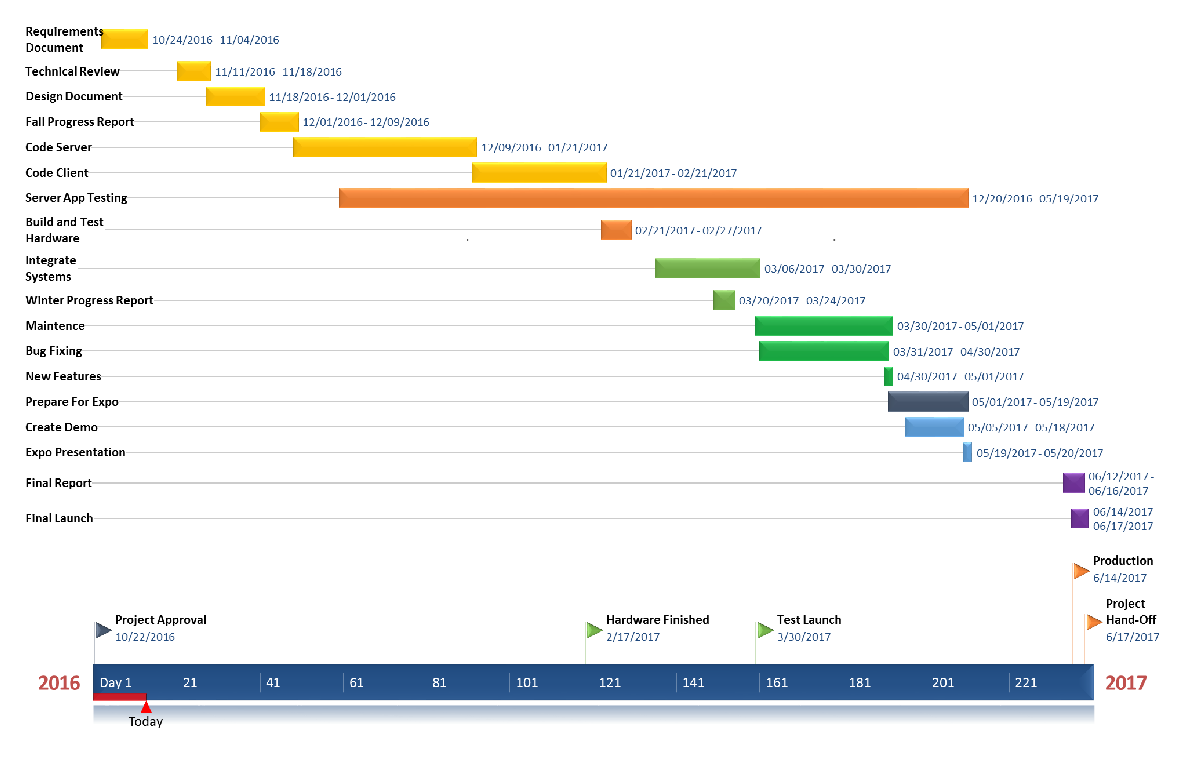
\includegraphics[width=\linewidth]{ganttchart.eps}
		\caption{A Gantt chart outlining the work to be done over the next nine months.}
		\label{fig:gantt}
	\end{figure}

	Figure \ref{fig:gantt} shows a gantt chart outlining our schedule from now until the first test rocket launch.
	Although the final rocket launch is on 23 June, all core systems of GS should be finished by the test launch in mid-May.

	\index{Specific requirements}
	\subsection{Specific requirements}

	\index{External interface requirements}
	\subsubsection{External interface requirements}
	\index{User interfaces}
	\subsubsubsection{User interfaces}
	Users will interact with GS by connecting via a web browser. The Raspberry Pi and other associated hardware,
	to be provided by the avionics team,
	will broadcast a wireless network that users will connect to and access GS through a web browser.
	From this page, users will be able to access the graphical display of the telemetry.
	
	\index{Hardware interfaces}
	\subsubsubsection{Hardware interfaces}
	GS will run on a Raspberry Pi broadcasting a wireless network. Users will connect to GS with their personal computers
	via the wireless network.

	Data is received from a serial interface using a protocol that will be determined by the avionics team.

	\index{System Features}
	\subsubsection{System Features}

	The stimulus for all specific requirements is receiving a telemetry packet. The specific responses to each telemetry packet are:
	\begin{itemize}
		\item GS will collect data from a serial interface using a yet-to-be-determined protocol designed by the High-Altitude Rocketry Team's avionics section.
		\item GS will log all telemetry in real-time to non-volatile storage so that it can be analyzed
		after the launch.
		The data from the serial port will be written to directly to non-volatile storage in order to limit
		the possibility of corruption.
		\item The graphical display shall be updated in real-time.
		\item Users will connect to GS and be able to view a visualzation of the telemetry in real-time.
		\item GS will support a live line graph visualization for altitude data.
		\item GS will have the ability to show the most recently recorded latitude and longitude in a numerical format.
	\end{itemize}

	\index{Performance requirements}
	\subsubsection{Performance requirements}

	\begin{itemize}
		\item When a new telemetry packet is received, GS will log the telemetry and update all visualizations in under one second.
		\item GS will support a minimum of 20 concurrent users.
	\end{itemize}



	\subsubsection{Design constraints}
	\index{Design contraints}
	\index{Contraints}
	\index{Raspberry Pi}
	GS will run on the hardware chosen by the avionics team at the beginning of the project.
	At a minimum, this hardware will be a Raspberry Pi 3 model B, which has a 1.2 GHz quad-core 64-bit ARM Cortex-A53 processor
	with 1 GB of SDRAM memory.

	\subsubsection{Software system attributes}

	\subsubsubsection{Reliability}
	\index{Reliability}
	In the event a GS process dies, a new process should begin and continue operation in under five seconds.

	\subsubsubsection{Robustness}
	\index{Robustness}
	If GS receives corrupted or otherwise incorrectly formatted telemetry, it should not crash.
	Additionally, the users should not be able to crash GS from the web interface.

	\subsubsubsection{Accuracy}
	\index{Accuracy}
	GS should not introduce any errors in the telemetry it recieves.
	Data should be logged and displayed with 100\% accuracy.



































\newpage
\section{Changes in Requirements}
The written requirements remained unchanged throughout the duration of the project.
























% CHAPTER
% DESIGN
\newpage


%	\pagestyle{empty}
%	\vspace*{2in}
	\section{Design}
	
%	\vspace{5mm}
	
%	\pagestyle{headings}
	
%	\newpage

	% Uncomment this to make the table of contents	

	\subsection{Introduction}

	\subsubsection{Identification}
	This document will provide and in-depth software design description of the Groundstation software package.
	
	\subsubsection{Date of Issue}
	This document is issued on December 2, 2016.
	At this time, the design of the software is complete, but no work has begun on the implementation.
	
	\subsubsection{Scope}
	This document will provide details about the Groundstation software package.
	The concerns of the software will begin when the telemetry is received via the serial port on the Raspberry Pi.
	Collecting the data from the rocket and converting it into a protocol readable through the serial port is the
	concern of the \ac{OSU} \ac{AIAA} High-Alititude Rocketry Team avionics section.
		
	\subsubsection{Stakeholders}
	The stakeholders of the Groundstation software package are members of the \ac{OSU} \ac{AIAA} High-Altitude Rocketry Team.
	The \ac{OSU} \ac{AIAA} High-altitude rocketry team is a group of multidisciplinary engineering students who are working to together to build the rocket.
	The stakeholders require the ability to:
	\begin{itemize}
		\item View the telemetry in real time in order to track the altitude and aid in recovery
		\item View the data graphically so that it is easy to understand
		\item Log the data so that it may be analyzed at a later date
	\end{itemize}

	\index{Structure view}
	\subsection{Structure View}
		
	
	
	% LOOK AT MY NEWELEMENT COMMAND EXAMPLEHERE
	

	\entityref{PC}
	{Interaction View - PC}

	\newentity
	{Albert Morgan}
	{Package Manager}
	{Subprogram}
	{
		The package manager will install, track, and update software dependencies on the server.
	}
	{
		Because Groundstation will be using Node and JavaScript for both the frontend and backend, \ac{NPM} will be used~\cite{npm}. \ac{NPM} has a large repository of both server-side and client-side JavaScript packages.
	}
	
	\index{Visualization}
	\index{JavaScript}
	\index{3.js}
	\index{Frontend}
	\index{WebGL}
	\newentity
	{Natasha Anisimova}
	{Frontend}
	{Component}
	{User Interface}
	{
		The frontend of the web server will create and display the information that it was given by the backend. Given
		that the information has to do with location
		(longitude, latitude, and altitude), a 3D display is preferred. The
		frontend will consist of programs using 3.js and WebGL to create the visualization necessary to quickly understand the
		location of the rocket.
	}

	\index{Backend}
	\newentity
	{Albert Morgan}
	{Backend}
	{Component}
	{
		The purpose of the backend is the facilitate communication between the rocket and the user.
	}
	{
		The backend takes care of all data collection, transformation, logging, and serving that data to the user.
		A Node server will handle reading the data from the serial port, transforming the data into JSON,
		storing the data, and making the data available to the user over the wireless network.
	}

	\index{Node}
	\index{Backend}
	\index{PHP}
	\index{Ruby}
	\index{Raspberry Pi}
	\newentity
	{Albert Morgan}
	{Node}
	{Subprogram}
	{Node is the software that runs the backend.}
	{
		The backend will run on Node. Several choices were considered to run the backend, particularly Node~\cite{node}, PHP~\cite{php}, and Ruby~\cite{ruby}.
		The backend was chosen two criteria:
		\begin{itemize}
			\item Speed. The backend will run on a Raspberry Pi, so speed is important to minimize the system resources used.
			\item Interoperability. The backend needs to work with multiple components, including the logging software, the data coming in from the serial port, and serving the frontend to the user.
		\end{itemize}
		Node uses an event driven architecture, which is ideal for reading data from the serial port.
		PHP and Ruby on Rails are both HTML preprocessors, so they don't get activated until the web site is requested.
		Node, on the other hand, runs continuously in the background and uses an event driven architecture.
		The event driven architecture is ideal for reading the data from the serial port.
		Additionally, Node much faster than either ruby or PHP.	
	}

	\newentity
	{Terrance Lee}
	{Serialport}
	{Library}
	{Node serialport library}
	{The Node serialport library allows us to transfer data from one device to another. }

	\index{Log}
	\index{JSON}
	\newentity
	{Albert Morgan}
	{Log}
	{Data store}
	{Store the data in non-volatile storage for later retrieval and update new connecting clients}
	{
		Groundstation will store telemetry in JSON format.
		The log should limit the possibility of the corruption of the data due to a programming error
		and make the data easily accessible for newly connecting clients.
		Several choices were considered for the logging, including relational databases, JSON documents, and logging the raw telemetry.
		
		A relational database would be unnecessary because the data does not have any relations that need to be tracked;
		each telemetry packet is an independent piece of information.
		Logging the telemetry as it comes in from the rocket would limit the possibility of corruption.
		A programming error in the JSON parsing routines could cause all of the data to be unusable.
		However, storing the data in JSON format would make it very easy for new clients that connect to the server in the middle of the rocket flight to be updated with all of the past data.
		Additionally, a JSON document would be easy to expand into a NoSQL database such as MongoDB~\cite{mongodb}.
		For this reason, the telemetry will be stored in a JSON format.
	}
	
	
	\newentity
	{Terrance lee}
	{JQuery}
	{Library}
	{Make it easier to use JavaScript on our website. }
	{Our main concern with JQuery is that it may have limited functionality.  JQuery has an extensive library, but if your website has a lot of customization in it, there is a chance of running into limited functionality with it.  There are two ways to counter this issue.  One is keep the website simple.  Our main focus is to collect data from the rocket and display it.  Keeping a simple website with that in mind should not be a problem.  The second way if we need to customize more than it can handle is by using raw JavaScript for the parts that are causing the issue.}
	
	\index{Visualization}
	\index{JavaScript}
	\index{User Interface}
	\index{WebGL}
	\index{Web browser}
	\newentity
	{Natasha Anisimova}
	{3.js}
	{Library}
	{3.js is a JavaScript 3D library used to create and display animated 3D computer graphics using WebGL.}
	{	Since the information about the rocket will be displayed by using a web browser through a local Wi-Fi network, 
		making sure the information is displayed on time and correctly is crucial. 3.js allows for easy and rapid development
		of WebGL applications, which means we can make the most of the specialized graphics hardware on the users'
		PCs.
	}


	\index{Rocket}
	\index{Longitude}
	\index{Latitude}
	\index{Altitude}
	\newentity
	{Natasha Anisimova}
	{Rocket}
	{Component}
	{Physical manifestation of the object being tracked.}
	{
		The rocket will have sensors attached to it that will transmit information about its altitude, GPS coordinates, and tilt.
		While the rocket is on its journey, the GPS signal will cut out due to the COCOM limit.
		Because of the COCOM limit, that the longitude
		and latitude will have to be calculated based upon the other information that is received. 
	}
	
	\index{Web server}
	\index{Raspberry Pi}
	\index{JSON}
	\index{Telemetry}
	\newentity
	{Albert Morgan}
	{Web server}
	{Part}
	{	The web server will serve three primary functions:
		\begin{itemize}
		\item Serve web pages to the clients
		\item Receive telemetry from the serial port and convert it into JSON
		\item Make the JSON data available to the clients
		\end{itemize}
	}
	{
		The web server needs to be stable so there is no data loss during the flight.
		Additionally, the web server should be as lightweight as possible to minimize the resource consumption on the Raspberry Pi.
		Groundstation will use the Apache~\cite{apache} web server.
		This web server was chosen over other options primarily for its stability.
		Apache uses a one-thread-per-connection model~\cite{nginx-vs-apache-our-view}, so if one thread crashes, it will not affect the rest of the connections.
		NGINX~\cite{nginx} was also considered. On large-scale servers, it is much more lightweight because it uses a many-connections-per-thread
		model.
		This allows NGINX to stay responsive even when there are thousands of connections.
		However, the number of connections will be small and the reuse of threads could reduce stability.
		For example, the thread serving the connection could crash and disconnect everyone using the software.
		Lighttpd~\cite{lighttpd} was also considered. Although Lighttpd is much more lightweight than Apache,
		it is not nearly as mature.
		Because stability is a primary concern, Apache was selected.
	}

	\begin{center}
	\begin{figure}[thbp!]
		\centering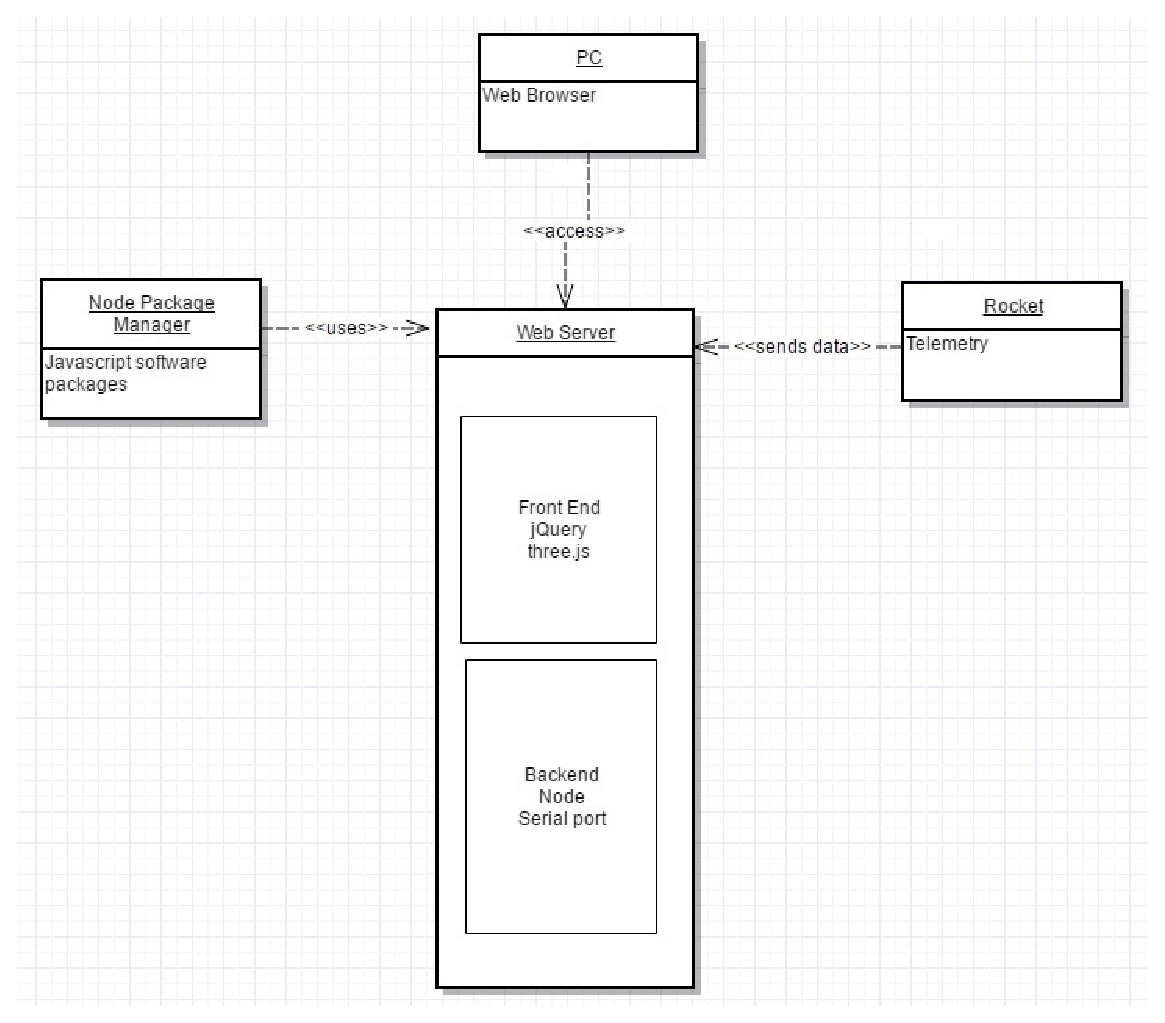
\includegraphics[width=170mm]{UMLdiagram1.eps}
		\caption{A UML diagram of what the web server is and how it is connected to everything else.}
		\label{uml4}
	\end{figure}
	\end{center}
	\clearpage
	\index{Web browser}
	\index{Chrome}
	\index{Edge}
	\index{Firefox}
	\index{Safari}
	\newentity
	{Albert Morgan}
	{Web browser}
	{Process}
	{The web server}
	{	The client will use a web browser to connect to the Groundstation web server and access the content.
		The web browser may be any of:
		\begin{itemize}
			\item Chrome version 54 or higher
			\item Edge version 14 or higher
			\item Firefox version 49 or higher
			\item Safari version 10 or higher
		\end{itemize}
		These browsers were selected to be supported because they represent the most recent versions of the most popular web browsers in use today.
	}

	\index{Web browser}
	\index{Web server}
	\newrelationship
	{Albert Morgan}
	{Web browser / Web server}
	{Connected}
	{The web browser connects to the web server over a WiFi network via the HTTP protocol.}
	
	\newrelationship
	{Natasha Anisimova}
	{Frontend / Backend}
	{Connected}
	{The Frontend will take what the Backend of the software gives it and use 3.js to create and display information to the user.}
	
	\newrelationship
	{Terrance Lee}
	{JQuery composition}
	{Composition}
	{JQuery will be used to make our PC Controls on the website}
	
	\newrelationship
	{Natasha Anisimova}
	{3.js}
	{Part of}
	{The JavaScript Library 3.js will be used with WebGL to create the frontend of Groundstation. Figure \ref{fig:4} goes through how 3.js is a part of the creation of the frontend}
	
	\begin{center}
	\begin{figure}[htbp!]
			\centering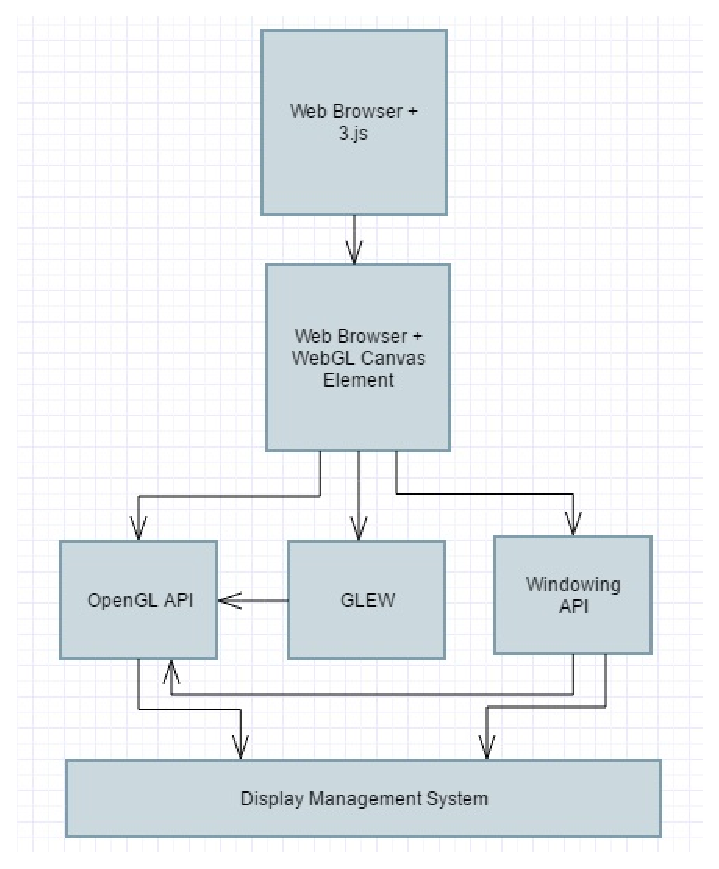
\includegraphics[width=110mm]{RelationshipDiagram.eps}
			\caption{A diagram of how 3.js is connected to WebGL and the frontend.}
			\label{fig:4}
	\end{figure}
	\end{center}
	\clearpage
	\index{Node}
	\index{Backend}
	\newrelationship
	{Albert Morgan}
	{Node / Backend}
	{Part of}
	{	Node is used by the backend to do the majority of the work.
		Node is responsible for receiving, transforming, logging, and sending the telemetry to the user.
	}
	
	\newrelationship
	{Albert Morgan}
	{Serialport use}
	{Use}
	{Node uses the serialport library to get data from the serial port.}
	
	\index{Log}
	\index{Backend}
	\newrelationship
	{Albert Morgan}
	{Log / Backend}
	{Part of}
	{
		The log is part of the backend, and will be written to by the backend and exist on the same device that runs the backend.
	}
	
	\newrelationship
	{Albert Morgan}
	{Backend / Rocket}
	{Connected}
	{The backend will retrieve data from the rocket through the serial port.
		The exact protocol used will be determined at a later date by the \ac{OSU} \ac{AIAA}
		High-Altitude Rocketry avionics team.
	}
	
	\newrelationship
	{Albert Morgan}
	{NPM / Frontend}
	{Connected}
	{NPM will be used to install all frontend software dependencies.}
	
	\index{NPM}
	\index{Backend}
	\newrelationship
	{Albert Morgan}
	{NPM / Backend}
	{Part of}
	{NPM is part of the backend, and will be used to update and install all backend software dependencies.}


	% INTERACTION SECTION
	\index{Interaction view}
	\subsection{Interaction View}
\newentity
	{Terrance Lee}
	{PC}
	{Component}
	{To be a tool to interact with the Raspberry Pi and the user.}
	{With the interaction of the PC and the Raspberry Pi our concern is the loss of connection due to the loss of the Wi-Fi signal.  The Raspberry Pi is just like any other Wi-Fi router and has the same issues that can drop signals.  The major issue we have to be concerned about is overheating.  We are going to be in New Mexico, out in the desert.  In Black Rock, NM we may experience temperatures up to 101 degrees.  We may be in a hotter area.  To counter this, we will have the ground station in an open area so that it can get plenty of air flow.  The second is that we will put in shade.  We will have to bring an umbrella or a tent.  This will allow the ground station to breath and stay cool.  The umbrella or tent will bring the temperature down as well.} 

	\newrelationship
	{Terrance Lee}
	{PC}
	{Component}
	{With the interaction between the website and the user we still need the PC as a tool. Our concern  in between these two is usability.  With that concern we want to make sure that everyone can understand how to navigate the website so that they do not get loss.  There are two things we want to focus on to counter this. The first thing is to use Krug’s first law of usability, the web-page should be obvious and self-explanatory.  When we make our website we need to make it so that the High-altitude Rocket team can get from point A to point B easily.   That way if they need to navigate multiple pages they won’t get lost.    The second is the “keep it simple” principle (KIS).  Doing this will help the Rocket team when they have to use anything on the page that they are on. If it is simple to use, then there is less of a chance of mistakes or misunderstandings.}
	\entityref{Rocket}
	{Structure View - Rocket}
	
	\entityref{Web Server}
	{Structure View - Web Server}
	
	\entityref{Web Browser}
	{Structure View - Web Browser}
	


	\newrelationship
	{Albert Morgan}
	{Telemetry Protocol}
	{Signal}
	{
		Once every second, the rocket will send a telemetry packet to the groundstation
		(the groundstation hardware, not the Groundstation software packagex).
		This packet will be received and transformed into a protocol that will be transmitted to the
		Groundstation software package via the serial port.
		The specification of this protocol will be determined by the avionics team at a later date.
	}

		
	\newrelationship
	{Albert Morgan}
	{JSON Protocol}
	{Signal}
	{
		Data will be stored in the log file and transmitted to the user as a list of JSON objects in the following format:\\


\noindent\{\\
\hspace*{.5cm}sensor: ...,\\
\hspace*{.5cm}value: ...,\\
\hspace*{.5cm}timestamp: ...\\
\}\\

		The JSON object has the following attributes:
		\begin{itemize}
			\item\textbf{Sensor}: This is the name of the sensor that the data is recorded from.
			This is an arbitrary string that uniquely identifies a specific sensor on the rocket.
			This string may be anything, and the user interface must understand which sensors provide which data.
			The specification of which strings correspond to which sensors will be done at a later date, after the protocol is defined.
			\item\textbf{Value}: This is the value that has been read off the sensor.
			The type of this data will depend on the specific sensor.
			\item\textbf{Timestamp}: This is the time and date that the data was received.
			This value is an integer representing the number of milliseconds that have elapsed since the epoch (January 1, 1970).
		\end{itemize}
	
			JSON objects will be transmitted to the client as a single object with a list of smaller objects inside. For example:\\

\noindent\{\\
\hspace*{.5cm}\{\\
\hspace*{1cm}sensor: altimeter,\\
\hspace*{1cm}value: 900,\\
\hspace*{1cm}timestamp: 00584747458945\\
\hspace*{.5cm}\},\\
\hspace*{.5cm}\{\\
\hspace*{1cm}sensor: tilt,\\
\hspace*{1cm}value: 4,\\
\hspace*{1cm}timestamp: 00584747458945\\
\hspace*{.5cm}\}\\
\}
}

	\index{Interface view}
	\subsection{Interface View}
	
	\newinterface
	{Natasha Anisimova}
	{3D View}
	{Displays the current location of the rocket.}
	{The user can interact with the view by using a mouse or track pad.}
	{
		The view will be a 3D environment that will resize as the user
		resizes the window of the web browser. If the user clicks and drags in a particular direction
		the 3D environment will move in that direction. If the user just moves the mouse without clicking, the mouse will move freely on the screen. To make orientation easier in this environment, there will be a set of buttons, shown in the figure below, that will have preset views readily available for the user. The top-most button will show a bird's eye view. The left button will show a three-fourths view facing the left side of the launch site. The right button will do the same as the left button except facing the right side of the launch site. Finally, the bottom button in this set will give a view that is directly aligned with the ground, or XZ plane, looking out into the horizon. With the help of these buttons, the user should never feel like they are unable to get back to looking at the journey of the rocket. The scroll button will zoom in and out, with the point of origin being the launch location of the rocket. Figure \ref{fig:1} shows camera view controls that will be located in the top right corner of the browser.
	}
	\begin{center}
	\begin{figure}[htbp!]
		\centering
\includegraphics[width=3.5cm]{cameracontrols.eps}
		\caption{A diagram of the camera view controls.}
		\label{fig:1}
	\end{figure}
	\end{center}


	\newinterface
	{Natasha Anisimova}
	{3D Environment}
	{Displays the current location of the rocket in the launch environment.}
	{The user can interact with the view by using a mouse or track pad.}
	{
		The 3D environment will consist of the topological map of the launch site (Spaceport America in New Mexico), with satellite images from NASA of the area mapped to it. If the user zooms past the point that the topological map covers, the ground will be displayed as a flat gray plane that goes on forever in every which way the ground would be. Since the rocket's goal is to reach 100,000 feet in height, labeling the different levels of the atmosphere that it enters would be helpful. Each level will be a transparent shade of blue, going from light to dark. Figure \ref{fig:2} shows the layers of the Earth's atmosphere.
	}
	\begin{center}
	\begin{figure}[htbp!]
		\centering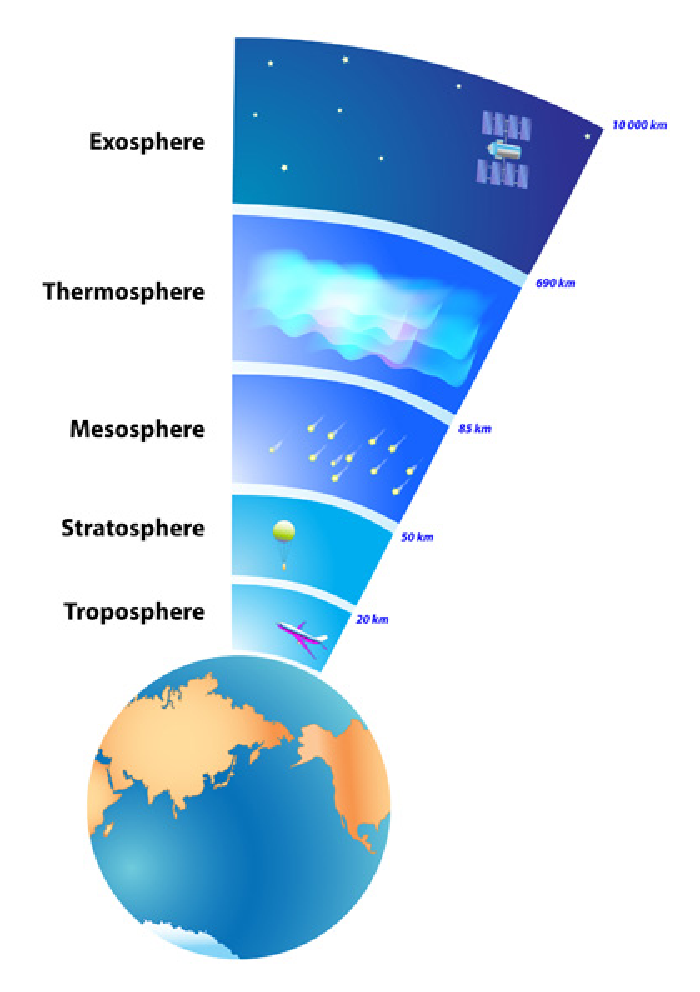
\includegraphics[width = 120mm]{earth-atmosphere-layers.eps}
		\caption{A diagram of the Earth's atmosphere.}
		\label{fig:2}
	\end{figure}
	\end{center}

%	Figure \ref{fig:2} Shows the layers of the Earth's atmosphere.
\newpage
	\newinterface
	{Natasha Anisimova}
	{Numerical Data}
	{Shows numerical data for the location of the rocket.}
	{The user can view or hide the table.}
	{
		Visual data can be hard to interpret without any numerical data to put it into perspective. Due to this, a table with the altitude, longitude, and latitude will be a part of the user interface. This table will be updated every time that a telemetry packet is received and given to the frontend of the web server.
		Figure \ref{fig:3} shows an example of how the table could be visible or hidden based off of what the user wanted.
	}
	\begin{center}
	\begin{figure}
		\centering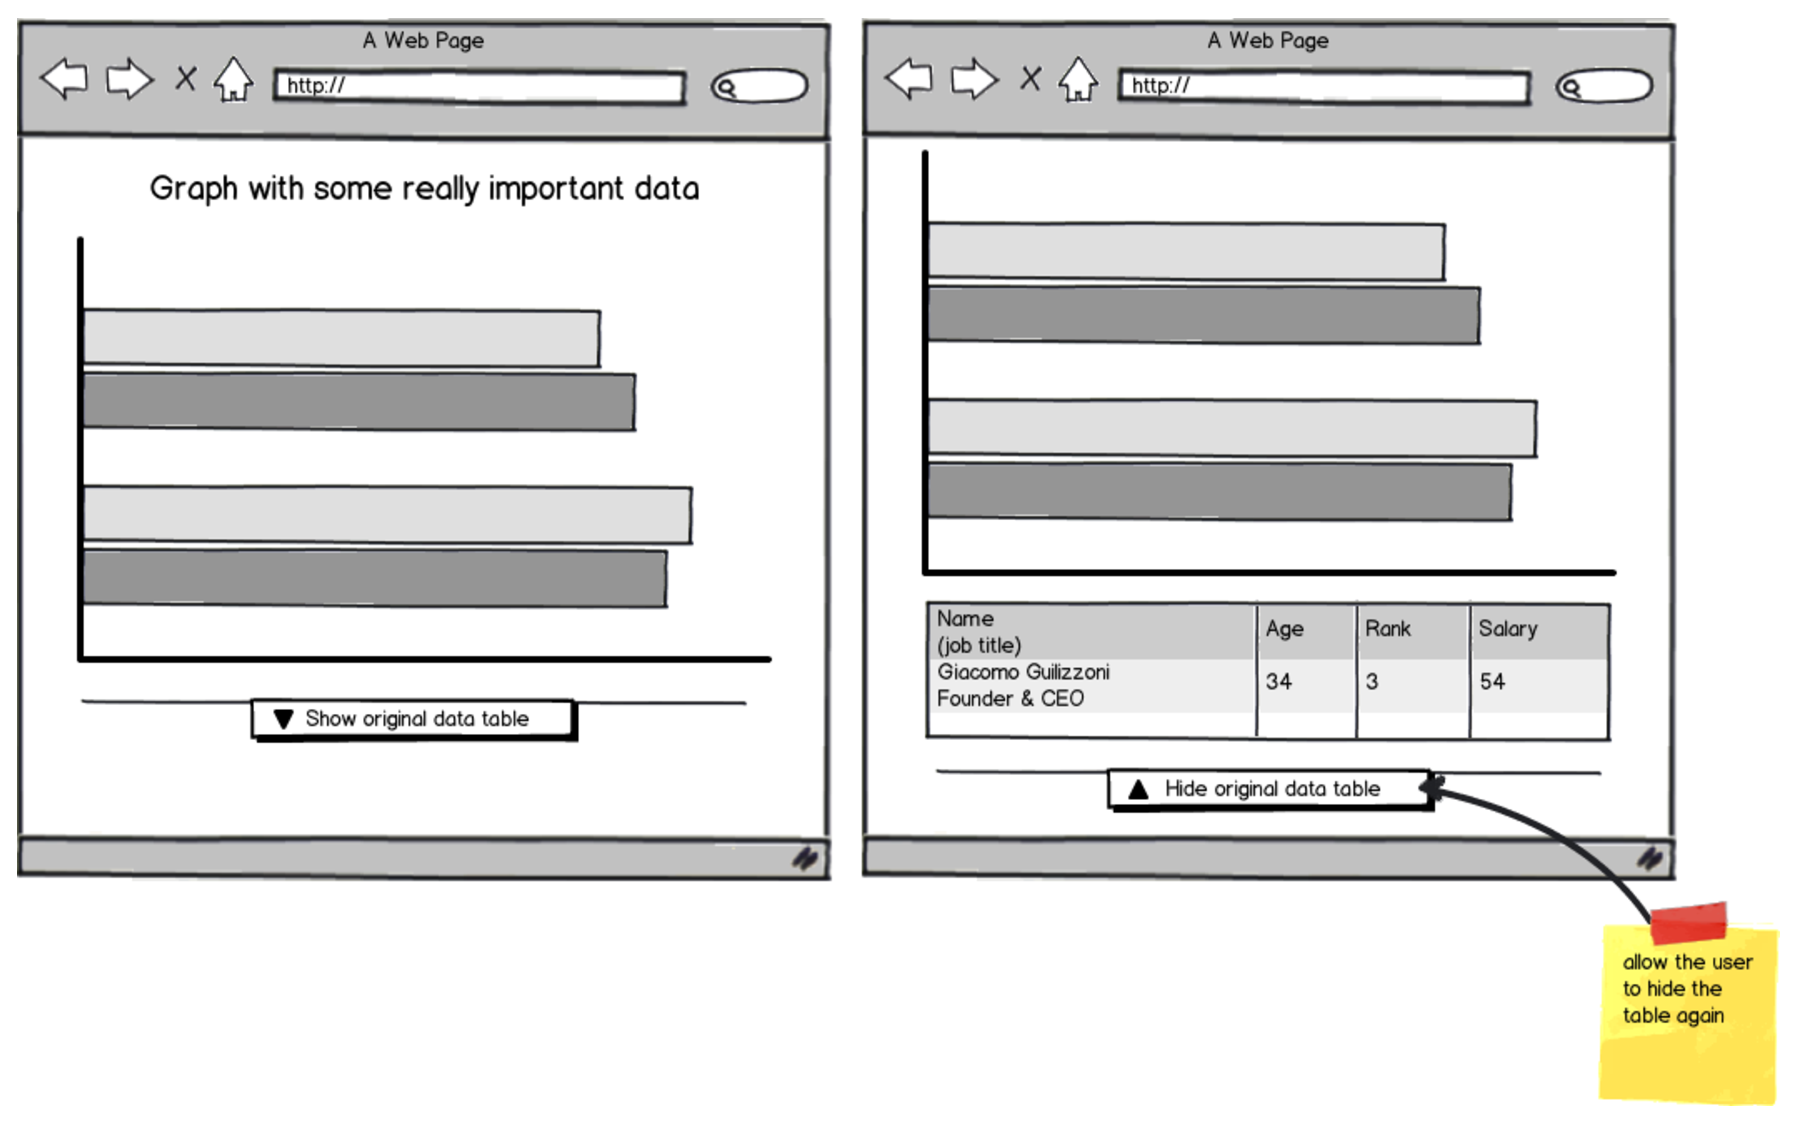
\includegraphics[width=\linewidth]{hideshowtable.eps}
		\caption{A diagram of how to show or hide a table.}
		\label{fig:3}
	\end{figure}
	\end{center}

\entityref{JQuery}
	{Structure View - JQuery}
    
\newrelationship
	{Terrance Lee}
	{JQuery interface}
	{interface}
	{ Our other concern with JQuery is the interface with the user. We want to build our dials, sliders or buttons using JQuery.  The concern is not whether or not it will work, but if it is right for the sub-teams.  We have at least five sub teams plus their members using them.  JQuery has a vast selection of PC controls. If we select the wrong setup for the team it may make it difficult for the teams to use. To counter this, we have to think about usability.  The first thing we should do is find data each team needs from the rocket.  Next find out if they are going to need PC controls. If so, then find out which ones would suit them best through user stories.  }	
	
   \index{Resource view}
	\subsection{Resource View}
    
     
   \newentity
	{Terrance Lee}
	{Math.Js}
	{Library}
	{Node Math library}
	{Our concern with Retrieval is loss of certain sensors.  Do to CoCom limits we lose the GPS sensor until it is under 1200 mph and under 60,000 feet. This will happen after apogee.  Also we lose accurate reading from the altimeter after 100,000 feet due to restrictions of the sensor itself.  It cannot read accurately after that height; it will just read a constant pressure until the rocket gets below that 100,000 feet. To counter act these loses we have other sensors like accelerometer and gyroscope which we can use physics and math formulas to get a location of the rocket.  With Math.js this allows us to use formulas and any other math equations to achieve this. }
     \entityref{Node}
	{Structure View - Node}
    
    \newrelationship
	{Terrance Lee}
	{Node}
	{Part of}
	{	Node is will allow us to store to the server while we are collecting the data. The data will stay on the server until we power it down.  This should allow us plenty of time to save it to our computers and hard drives.  This allows us time for resets due to software issues as well.  
		}
	
	
	\subsection{Revisions}


	\index{Log}
	\index{CSV}
	\newentity
	{Albert Morgan}
	{Log Revised}
	{Data store}
	{Store the data in non-volatile storage for later retrieval and update new connecting clients}
	{
		Groundstation will store telemetry in CSV.
		The log should limit the possibility of the corruption of the data due to a programming error
		and make the data easily accessible for newly connecting clients.
		Several choices were considered for the logging, including relational databases, JSON documents, CSV, and logging the raw telemetry.
		
		A relational database would be unnecessary because the data does not have any relations that need to be tracked;
		each telemetry packet is an independent piece of information.
		Logging the telemetry as it comes in from the rocket would limit the possibility of corruption.
		JSON format would make it easy to import the data into a running Node application, but may become corrupted if the program halts
		unexpectedly.
		Additionally, programming error in the JSON parsing routines could easily cause all of the data to be unusable.
		CSV format will be used for two reasons.
		First, there are no special ending characters, such as curly braces, that need to be inserted at the end of objects.
		The data will be easily readable even if the process halts unexpectedly and isn't able to finish formatting the log.
		Second, CSV files are easy to import into applications such as Microsoft Excel.
		Our teammates will be able to easily load up the data into an application of their choice for analysis after the launch.

	}


	\index{Web Server}
	\index{Raspberry Pi}
	\index{JSON}
	\index{Telemetry}
	\index{Node}
	\newentity
	{Albert Morgan}
	{Web Server Revised}
	{Part}
	{	The web server will serve three primary functions:
		\begin{itemize}
		\item Serve web pages to the clients
		\item Receive telemetry from the serial port and convert it into JSON
		\item Make the JSON data available to the clients
		\end{itemize}
	}
	{
		The web server needs to be stable so there is no data loss during the flight.
		Additionally, the web server should be as lightweight as possible to minimize the resource consumption on the Raspberry Pi.
		Groundstation will use the Node's~\cite{node} built-in web server.
		This web server was chosen over other options primarily for its stability.
		Apache uses a one-thread-per-connection model~\cite{nginx-vs-apache-our-view}, so if one thread crashes, it will not affect the rest of the connections.
		NGINX~\cite{nginx} was also considered. On large-scale servers, it is much more lightweight because it uses a many-connections-per-thread
		model.
		This allows NGINX to stay responsive even when there are thousands of connections.
		However, the number of connections will be small and the reuse of threads could reduce stability.
		For example, the thread serving the connection could crash and disconnect everyone using the software.
		Lighttpd~\cite{lighttpd} was also considered. Although Lighttpd is much more lightweight than Apache,
		it is not nearly as mature.
		Finally, we considered Node's built-in web server.
		Node's built-in web server would allow us integrate the rest of our code (which is written in Node) with the web server.
		Because we are already writing a lot of code based on the Node framework,
		writing the web server in the same language (JavaScript) will lower the time taken to develop.
		The extra time and ease of use will allow us to devote more time to testing and stability,
		effectively negating the benefit of using a more mature platform such as Apache.
		Finally, not using another piece of software for the web server will lower the time and effort it takes to install the software.
		This may be important if the software needs to be installed quickly on launch day.

		For all of the reasons listed, the built-in Node web server was selected.
	}




	\newrelationship
	{Albert Morgan}
	{JSON Protocol Revised}
	{Signal}
	{
		Data will be stored in the log file and transmitted to the user as a list of JSON objects in the following format:\\


\noindent\{\\
\hspace*{.5cm}id: ...,\\
\hspace*{.5cm}latitude: ...,\\
\hspace*{.5cm}longitude: ...,\\
\hspace*{.5cm}accelerometer\_x: ...,\\
\hspace*{.5cm}accelerometer\_y: ...,\\
\hspace*{.5cm}accelerometer\_z: ...,\\
\hspace*{.5cm}yaw: ...,\\
\hspace*{.5cm}pitch: ...,\\
\hspace*{.5cm}roll: ...,\\
\hspace*{.5cm}timestamp: ...\\
\}\\

		The JSON object has the following attributes:
		\begin{itemize}
			\item\textbf{id}: This is the id of the rocket component that the packet comes from. There are two stages to the rocket: the booster and the sustainer, and each of them will be sending packets.
The id field will inform client which part of the rocket this packet comes from, '0' for the booster, and '1' for the sustainer.
			\item\textbf{timestamp}: This is the time and date that the data was received.
			This value is an integer representing the number of seconds that have elapsed since the epoch (January 1, 1970).
			\item\textbf{other}: All other fields represent individual sensor readings. The units of these fields will be metric, except for angles, which will be encoded as degrees.
		\end{itemize}
}
	\index{Visualization}
	\index{JavaScript}
	\index{3.js}
	\index{Frontend}
	\index{WebGL}
	\newentity
{Natasha Anisimova}
{Frontend}
{Component}
{User Interface}
{
	The frontend of the web server will create and display the information that it was given by the backend. Given
	that the information has to do with location
	(longitude, latitude, and altitude), a 3D display is preferred. The
	frontend will consist of programs using 3.js and WebGL to create the visualization necessary to quickly understand the
	location of the rocket. There is a problem with the data being sent and having a 3D display. The Avonics team has
	a 3-axis gyroscope and the GPS will only be turning on at apogee. Gyroscopes tend to drift on their own so the direction
	of the rocket's flight will not be one-hundred percent accurate until the GPS. Having a simple 2D graph of the rocket's
	flight path to fall back on would be helpful in case the GPS does not turn on.
}
	

\subsection*{Revision History}
\vspace{0.5cm}
\begin{tabular}{l | l | l}
Name & Section Title & Date\\ \hline
Albert Morgan & Log Revised & 2017-02-15\\
Albert Morgan & Web Server Revised & 2017-02-15\\
Albert Morgan & JSON Protocol Revised & 2017-02-15\\
Natasha Anisimova & User Interface Revised & 2017-02-17\\
\end{tabular}

	%\allowdisplaybreaks
	\clearpage
	\newpage
	\subsection{Glossary}
		\begin{itemize}
		\index{Accuracy}
		\item \textbf{Accuracy:} The absence of errors in the telemetry GS receives, logs, and displays.
		\index{Binary data}
		\item \textbf{Binary data:} Telemetry that represents one of two states, for example, ``stage 2 activated'' and
		``stage 2 not activated.''		
		\index{COCOM limits}
		\item \textbf{COCOM limits:} The \ac{COCOM} limits apply hard limits to the speed and altitude of a GPS device.
		If a device exceeds these limits, it will stop providing GPS data.
		This is done to ensure that the device cannot be used as a missile.		
		\index{Corruption}
		\item \textbf{Corruption:} The process by which data is altered or made unreadable.
		\index{Crash}
		\item \textbf{Crash:} A software crash; the event in which a piece of software ceases operation unexpectedly.
		\index{Die}
		\item \textbf{Die:} A process dies when it ceases operation and is removed by the operating system.
		The difference between dying and crashing is that a crash may cause the program to become non-responsive,
		whereas dying causes the process to end.
		\index{Groundstation}
		\index{GS}
		\item \textbf{GS:} Groundstation, the name of our software.
		\index{Graphical display}
		\item \textbf{Graphical display:} Data that is displayed using a visualization.
		\index{Live}
		\item \textbf{Live:} Updated in real-time.
		\index{Non-volatile storage}
		\index{Storage}
		\item \textbf{Non-volatile storage:} Storage that will not be erased when the system is powered down.
		For example, a hard drive or flash storage.
		\index{Page}
		\item \textbf{Page:} A web page that users of GS may connect to in order to view the telemetry.
		\index{Process}
		\item \textbf{Process:} A running program on a computer.
		%\index{Lean angle}
		%\item \textbf{Lean angle:} The angle relative to the vertical that the rocket is currently traveling.
		\index{Raspberry Pi}
		\item \textbf{Raspberry Pi:} A small, inexpensive computing platform.		
		\index{Real-time}
		\item \textbf{Real-time:} Each telemetry datum received from the rocket must be processed and
		displayed in under one second.
		\index{Redundant sensors}
		\item \textbf{Redundant sensors:} Two or more sensors that provide the same type of data.
		\index{Reliability}
		\item \textbf{Reliability:} In the event of a software crash, the Groundstation software should automatically
		start and begin all normal functions in under five seconds.
		\index{Robustness}
		\item \textbf{Robustness:} In the event that GS receives data that is garbled or otherwise does not adhere
		to the protocol, it must continue to receive and display data and not break the real-time requirement.
		\index{Storage}
		\item \textbf{Storage:} A device where data is logged.		
		\index{Telemetry}
		\item \textbf{Telemetry:} Data received from the rocket while the rocket is in flight.
		\index{Telemetry packet}
		\index{Packet}
		\item \textbf{Telemetry packet:} The rocket will send a telemetry update once per second. Each one of these updates is a ``telemetry packet.''
		\index{Vizualation}
		\item \textbf{Visualization:} Information or data, transformed into an visual context.
		\index{X, Y, Z coordinates}
		\item \textbf{X, Y, Z coordinates:} A three coordinate system that pinpoints a point in 3D space.
		\index{XZ plane}
		\item \textbf{XZ plane:} A plane extending in the XZ directions. I.e., parallel to the ground.
	\end{itemize}















% CHAPTER
% TECH REVIEW










\newpage
\section{Tech Review}
	\subsection{Web Server}
	\index{Web Server}
	This section will describe the various options for the web server. Author: Albert Morgan.

	\subsubsection{Apache}
	\index{Apache}
	\index{Web Server}
	% Advantages:
	% Powerful module system	
	Apache is the most popular web server option, with over 50\% of the market share~\cite{apache-usage-statistics}.
	Apache uses a powerful and flexible module system that allows for a variety of different behaviors~\cite{apache-vs-nginx-practical-considerations}.
	Each connection to an Apache server spawns a new thread or process, depending on which modules are used.
	This feature has advantages and disadvantages.
	Because each connection spawns a new thread, if the thread serving one connection crashes, it will not affect the other connections.
	However, because each connection spawns a new thread, the overhead for that thread must be paid for each new connection.

	\subsubsection{NGINX}
	\index{NGINX}
	\index{Web server}
	% NGINX advantages:
	% fast processing
	% concurrency (don't need this, though)
	% resource efficiency
	% responsiveness
	NGINX is 2\textsuperscript{nd} most popular web server on the Internet~\cite{nginx-usage-statistics}.
	Web servers such as Apache that use a one-thread-per-connection model can have problems with large number of simultaneous connections, an issue known as the C10k problem~\cite{apache-vs-nginx-practical-considerations}~\cite{c10k-problem}.
	NGINX solves this issue by having one thread serve many connections.
	This approach reduces the overhead caused by spawning so many threads, and makes NGINX very lightweight and scalable~\cite{nginx-vs-apache-our-view}.
	
	\subsubsection{Lighttpd}
	\index{Lighttpd}
	\index{Web server}
	Lighttpd, pronounced ``lighty'', is a web server that is optimized for low memory footprints and fast response.
	It is optimized for serving a large number of concurrent keep-alive connections, such as serving high-volume AJAX driven web sites~\cite{lighttpd}. Many web sites use lighttpd for static content delivery while using another web server, such as Apache,
	for dynamic content~\cite{powered-by-lighttpd}.

	\subsubsection{Conclusion}
	All three web servers listed above have advantages for this project.
	Apache's one-thread-per-connection approach increases stability.
	NGINX and Lighttpd are both lightweight, which is important for running an application on a low-power system like a Raspberry Pi.
	However, Groundstation does not have to support more than 20 concurrent users, so the memory and processor savings for choosing a lightweight option will be minimal.
	Additionally, stability is a primary concern of the High-Altitude Rocketry Challenge.
	For these reasons, we recommend Apache.


	\subsection{Web Backend}
	This section will describe the options for the web backend. Author: Albert Morgan.
	
	\subsubsection{Node}
	\index{Node}
	\index{V8}
	\index{JavaScript}
	\index{Google Chrome}
	\index{Chrome}
	Node allows web backends to be written in JavaScript using V8, the same JavaScript engine that powers Google Chrome~\cite{node}.
	The client side of the web application will certainly use JavaScript, and writing the backend  in JavaScript as well will reduce the overhead of learning and programming in new languages.
	Additionally, because JavaScript would be used on the front-end and backend, it may be possible to reuse code between these two systems.
	
	Node uses an event driven architecture, and is built to work with \ac{JSON} data.
	With Node, is it easy to create a web application that response to small events and sends small bits of data to the client~\cite{event-driven-architecture-node-js}.
	Because Node uses JavaScript, it integrates naturally with \ac{JSON}.
		
	Benchmarks show that Node is over 5 times as fast as PHP, even when using just-in-time compilation~\cite{comparing-node-vs-php-performance}.
	
	\subsubsection{PHP}
	\index{PHP}
	PHP has been around the web since 1994 and is used in over 80\% of web sites today~\cite{history-of-php}~\cite{usage-of-server-side-programming-languages-for-websites}.
	Given its maturity and wide adoption, there are a lot of packages, documentation, and example available for developers.
	PHP's primary advantage is the ease in which is can be incorporated into an static webpage.
	Using PHP tags, HTML and PHP code can be intertwined seamlessly.
	
	\subsubsection{Ruby}
	\index{Ruby}
	Ruby is an open source programming language designed for simplicity and productivity~\cite{ruby}.
	It is well-known on the web as part of the framework Ruby on Rails, which allows for embedded Ruby to be inserted directly into HTML~\cite{getting-started-with-rails}.
	However, compared to PHP, Ruby on Rails has a steep learning curve.
	Ruby's syntax can be hard for a beginner to read, and it draws some concepts from functional programming, which can be difficult for a new user~\cite{ruby-on-rails-vs-php-the-good-the-bad}.	

	\subsubsection{Conclusion}
	Node is fast, which is important for the Groundstation server, which will run on a Raspberry Pi.
	Node also uses an event driven architecture, which is perfect for our software. Data will be received at regular intervals and need to be pushed out the clients quickly. For these reasons, we recommend using Node.


	\subsection{Logging}
	\index{Logging}
	\index{Telemetry}
	\index{Data}
	This section will describe how the telemetry will be stored. Author: Albert Morgan.
	\subsubsection{Raw data}
	\index{Raw data}
	The simplest logging method is to save the raw data stream to a file as it comes in.
	This method would be very low cost, in terms of development time, processing, and memory usage.
	The data would simply be read from the serial port and saved to a file, where it could be reconstructed at a later time.
	Saving the data at this point, before any processing is done, will reduce the chance of any corruption.
	
	\subsubsection{JSON}
	\index{JSON}
	\ac{JSON} is a data format that is easy for both machines and humans read and write.
	The telemetry may be stored after it is transformed from its raw form from the serial port to \ac{JSON}.
	The server will already be converting the raw data to \ac{JSON} in preparation to send it to the client, so there will be no additional overhead in the conversion.
	However, it is likely that the \ac{JSON} data will take up more space than the raw data due to additional formatting, so it will take up more space in the storage media~\cite{json}.
	
	\subsubsection{Database}
	\index{Database}
	\index{SQL}	
	Storing the telemetry in a database as it comes in will allow for fast random-access reading and writing of the data.
	This would allow the server to easily grab a certain subset of the data.
	For example, the server could send the client only data that was generated in the last 2 minutes, or data that comes off of one particular sensor.
	Data could easily be retrieved using queries in a language such as SQL.
	
	\subsubsection{Conclusion}
	Because the system only needs to store data from a single launch, the size of the data set will be relatively small.
	The overhead of sending all of the data would be minimal, so the benefits of using a queryable database would be small.
	In the event that the system goes down, it would need to start back up again and begin operation very fast.
	Storing the data in \ac{JSON} format would allow the data to be quickly loaded back into memory without significant processing.
	Additionally, if the data is stored in \ac{JSON} format, the server would not need to keep the entirety of it in memory to serve it to a connecting client, freeing up resources on the Raspberry Pi.
	For these reasons, we recommend that the data be logged after it is converted into \ac{JSON} format.

	\subsection{Data Visualization}
	\index{Data Visualzation}
	This section will describe the various options for the data visualization. Author: Natasha Anisimova.
	
	\subsubsection{2D-Representation}
	2-dimensional representations of maps are usually equal in the x and y dimensions~\cite{2d-is-better-than-3d}. 
	Graphs and charts are representations that most users are comfortable with, but they can also be a little dull.
	For displaying the location of a land-bound vehicle or person, a 2D graph is useful~\cite{2ds-company-3ds-a-crowd}. 
	The ground can be viewed as a 2D plane ~\cite{2d-and-3d-presentation-of-spatial-data}.
	With a rocket the altitude, latitude, and longitude has to be taken into account and displayed. 
	The most important aspects of the software project are to find the rocket's location in the end and to be able to tell 
	if it reached the team's one-hundred-thousand-foot goal. 
	
	\subsubsection{3D-Representation}
	2-dimensional topographic maps are hard to read if one has not had a lot of experience with them. 
	Considering that most of the team will be mechanical engineer,s and no earth science majors will be participating, a 
	3-dimensional map makes more sense. 
	Cartographers in the past decade have shifted to creating 3D perspective maps. 
	These types of maps are more expensive and time intensive to produce. 
	The extra time that is put into the visualization makes it more appealing to the readers~\cite{evaluating-the-effectiveness-of-2d-vs-3d-trailhead-maps}. 
	The 3D representation is easy to visualize and understand ~\cite{3d-represenation-for-software-visualization}.
	
	\subsubsection{Numerical Display}
	A numerical display is often used when looking for the longitude and latitude of a specific point on a map. 
	It would also be useful when displaying the highest altitude of the rocket ~\cite{data-display}. 
	The numerical display is a number that would constantly be reviewed and needed. 
	A graph can display the data, but it would still take a second to get that information. 
	Having a table will show all the most crucial aspects of the project with the values would make the webpage much more usable.
	
	\subsubsection{Conclusion}
	3D visualization for the location of the rocket as well as a small numerical display is the best way to go. 
	Professor Mike Bailey has created software that can create and extract the topology of a certain area, 
	making it much more manageable. 
	The High-Altitude Rocketry team will only need the topology data of Lucerne Dry Lake area of the Mojave Desert. 
	The images for the area can be pulled from NASA's website, and from there they can be texture mapped to the topology. 
	The numerical display will be used to give a more accurate and direct way of giving the data to the users. 
	
	\subsection{User Interface Interaction Model}
	\index{User Interface Interaction Model}
	This section will describe the various options for the user interface interaction model. Author: Natasha Anisimova.
	
	\subsubsection{Unity}
	\index{Unity}
	Unity 3D is an engine, not so much an application. 
	Groundstation software is going to be used by about thirty to forty people, if not more, and most of them would not have the
	Unity3D Web-Player installed. 
	Unity is a game development tool, and since this project is focusing on just creating a useful visualization of the 
	data that is collected, Unity is not suitable for this particular case ~\cite{unity}.
	
	\subsubsection{OpenGL}
	\index{OpenGL}
	OpenGL has one of the fastest languages to develop with, C++. 
	Double buffering also solves any problems with the program being in the middle of plotting data and the user getting
	a black screen. 
	Instead it shows the old frame until the new one is ready to be displayed. 
	Unfortunately, OpenGL does not run on the web ~\cite{why-you-should-use-webgl}.
	
	\subsubsection{WebGL}
	\index{WebGL}
	WebGL is the Javascript API that allows you to create 3D graphics in a browser. 
	Three.js is a tool used on top of WebGL, making it easier to create those 3D graphics. 
	Three.js is used when creating more complicated 3D scenes (textures, models, and rendering). 
	Several different types of browsers support it as well, from Desktop Opera to Firefox and Chrome. 
	WebGL is also the easiest 3D application to use, as well as the best tested and documented ~\cite{webgl-best-practices}. 
	Performance-wise it is also very fast even though programs are written in JavaScript. 
	
	\subsubsection{Conclusion}
	\index{WebGL}
	\index{OpenGL}
	WebGL is the most fitting choice to go with for this project.
	OpenGL is not supported by web browsers, while Unity is not as widely readily supported by web browsers as WebGL.
	The WebGL application can be used while still having the comfortable environment of the web development
	environment that HTML and JavaScript have to offer ~\cite{why-use-webgl-for-graphics-research}. 
	While there is a high learning curve, there is plenty of support for it at OSU as well as information on the web.
	The only major downside is that Internet Explorer, before 2013, does not support it, which is used by few and 
	far in between ~\cite{internet-ex}. 
	WebGL is supported by mobile devices if the software is expanded to them in the future.
	
	
	\subsection{User Interface Organization}
	\index{User Interface Organization}
	This section will describe the various options for the user interface organization. Author: Natasha Anisimova.
	
	\subsubsection{Paper Prototypes and User Interviews}
	In order to understand what are users are most comfortable with, it would be most cost effective and time efficient
	to create paper prototypes ~\cite{what-is-prototyping}. 
	A small sample of the High-Altitude Rocketry Team could be taken through a user study where we would try and figure
	what would work. 
	Feedback would be taken then and there.
	In some cases the feedback could be implemented quickly into the paper prototypes so that the user could see how it
	would affect the layout.
	
	\subsubsection{Flight Simulator Displays}
	A lot of flight simulator games efficiently display the information of the planes' or rockets' location, altitude,
	velocity, and status.
	Simulators are often able to do this with various dials on either side of the screen, much like a dashboard of a car.
	Having a recognizable display for the users would greatly reduce any misunderstandings that could occur ~\cite{flight-simulation-in-aerospace}. 
	Units and dials would be labeled for clarity. 
	Colors would be used to help emphasize important goals and perhaps how close they are to being reached.
	
	\subsubsection{Finnish Astronautical Society}
	The Finnish Astronautical Society has launch several different rockets since 2011 and successfully displayed the
	data that they have received from the rockets while they have been in space. 
	As mentioned on their website, most of the data is streamed to a ground station in real-time using a radio link and
	then from there onto an Internet server ~\cite{real-time-rocket-telementry-experiment}. 
	Their solution to the problem of keeping track of their rocket is very similar to what we have planned, except that they
	have a few different sensors and equipment.
	They have considerably more information about all their launches on their website, making it a bit cluttered, but the 
	content of their website is something that would be useful to follow.
	
	\subsubsection{Conclusion}
	For the organization of the user interface it would be useful to pull inspiration from websites or implementations
	that already exist but also have the freedom of easily changing it and being creative. 
	The paper prototypes would be useful for making sure that the software is easily tailored in the early stages of the 
	web page. 
	We have currently been pulling user stories from the team in order to know what would be most important for them to 
	see on the web page. 
	Continuing with that trend, we can continue to create the webpage with their feedback. 
	This would also ensure that they are not shocked or bewildered when seeing the final product before the launch date
	or on site.
	
	\subsection{Retrieval}
	\index{Retrieval}
	This section will compare programming languages for retrieving telemetry from the serial port. Author: Terrance Lee.
   	\subsubsection{C}
   	\index{C}
   	The C language has an extensive library which has many choices we can use. 
	The main one for the sensors is the extensive math.h library. 
	It allows us to do any math functions. Plus we can do error conditions in our code if needed. 
	When it comes to references, C has many. 
	Since C has had a couple of major programs, for example, Unix was rewritten in C in 1973 many people and companies have
	used C~\cite{history-of-unix-part-i}.
	This has allowed many references including the Internet, books, and instructors. C's disadvantage is that it is a very low level language and can be security flawed.

	\subsubsection{C++}
	\index{C++}
   	The C++ library is just as extensive as the C library except that it has made it so that it can be supported in an
	object oriented programming language. 
	For example, it has to bring out a cmath library so it works with C++.
	C++ is not as old as C. For example, in 1998 an ANSI/ISO standard for C++ was adopted~\cite{c-programmers-reference}.
	It is a favorite to many because of its object oriented programming (OOP). 
	Also, since it is OOP it is easier to write than C, but you have a lot more to learn. 
	That is its disadvantage: no developer can use its entire set of code that C++ provides.
	It would take an extremely long time. Just like C, there are many resources for C++ out there if we run into a problem.

	\subsubsection{Python}
	\index{Python}
   	The Python library is very extensive. 
	The new Python version 3.6 has about 37 main libraries which is sub-sectioned so that when you program you can be more specific~\cite{the-python-standard-library}.
	The main libraries that we need are the data types, numeric, and the mathematical modules. 
	When it comes to references, it seems that Python users understand that many schools do not have a class for it. 
	For example, when I was researching the libraries it had a reference page for the library. 
	Especially when it comes to the Internet, there are a lot of references to help if you run into issues with coding in Python.
	Python's disadvantage is that it is not popular. 
	Not many companies have given it a chance yet, and it has not had a big breakthrough.  
  
   	
   	\subsubsection{Conclusion}
   	All of these options are great. They all have extensive libraries and have great references. 
	If we run into any issues we have plenty of references online, as well as books and actual people we know that we can connect
	with and speak to about it. 
	We did some extra research and spoke to instructors and people that have used data collecting software in their career field
	before. 
	We asked them which language they preferred. 
	We got mixed results when it came to which one was the best language to use. 
	We believe that was because everyone has their favorite language that they prefer. 
	
   	We decided that the best language to use for the retrieval of data would be C. 
	It meets all of the criteria and beyond. 
	It has all of the libraries that we would need to retrieve the data from the sensors on the rocket. 
	If we lose GPS from a sensor we can still calculate the position of the rocket with those libraries as well. 
	With the amount of resources and references that are available to C, if we have an issue we should be able to find the solution
	to our problem quickly so that we do not get stalled on it for long.  
    
    \subsection{Interaction Modes}
    \index{Interaction Modes}
 	Support needs to be given for an interaction mode, PC or mobile, so that the High-Altitude Rocketry team can see the data. Author: Terrance Lee.

   	\subsubsection{PC}
   	\index{PC}
   	The PC interaction mode is the most available to the teams. It has the largest screen size and it has the most
	flexibility when coding. The disadvantage with the PC is that it is larger than mobile so the team will have to carry it around. 
	It can use up more power than the mobile too, but the battery can be more robust.

   	\subsubsection{Mobile}
   	\index{Mobile}
   	The mobile mode is also available to most of the people on the team as long as they have a smart phone. 
	The mobile option will give them a lighter option to carry around and will not waste as much power. 
	The disadvantage is that it will have a smaller screen and we have less flexibility when coding.  
	We will not have cell service when we are out at location.

   	\subsubsection{PC and Mobile}
    \index{PC}
    \index{Mobile}
    The third option is using both the PC and mobile. 
	With this option we will have all the advantages of both. 
	We will still have a disadvantage which is that we will have to program in multiple languages and formats. 

   	\subsubsection{Conclusion}
   	With the PC, once the team gets the information they will be able to save it right there on their team computers and move it
	easily through USB or other devices. 
	With mobile, our biggest issue is not the programming but the lack of cell service.
	Without cell service, if the team wants to look at any data they are reliant on the Raspberry PI Wi-Fi only. 
	That is not going to be on all the time, either. 
	If we use both, it has to be as a stretch goal because of the time constraints.  

   	The best option for this series that we would recommend would be to use the PC for the interaction mode. 
	It is reliable, most available, flexible when coding, and has a large screen size. 
	If multiple people are looking at the screen, they are pushing each other out of the way to see it. 
	When it comes to carrying it around, most of us have a computer bag and can carry it around that way. 
	That is not that big of a drawback. 
	With the power issue, we plan on bringing a power generator with us to the launch site, which the power plug for most computers
	are compatible with. 
	That should not be that big of an issue because we only need to have the computers on for launch and test launch.
	
    \subsection{Toolkit to generate the User Interface (UI)}
    \index{User Interface}
    \index{Toolkit to generate the User Interface}
 	For the toolkits to generate the UI, the options are Prototyping toolkits, jQuery UI, and the Dojo toolkit.
	These are all part of the top ten JavaScript Web UI Libraries, Frameworks and Toolkits~\cite{10-javascript-web-ui-libraries-frameworks-and-toolkits}.
	Author: Terrance Lee.

   	\subsubsection{Prototype UI}
   	\index{Prototype UI}
   	Our first option is the Prototype UI toolkits. 
	Their advantages are that they are reliable and have the functionality for our purpose. 
	The Prototype UI toolkits will allow us to generate the UI we want and has great documentation.
	The disadvantage is that they cost money. 
	The cheaper they are the less functionality, and the more expensive the more functionality. 
	The best one we found was called Mockplus, but its biggest disadvantage besides money is that it has a lack of responsive design
	features~\cite{pros-and-cons-of-four-prototyping-tools}.
	One big advantage is that ease of use due to its drag and drop feature.

   	\subsubsection{jQuery}
   	\index{jQuery}
   	The second option is jQuery. jQuery is free to use, easy to use, and has great documentation.
	One disadvantage with jQuery is that it has limited functionality in some cases~\cite{jquery-disadvantages-and-advantages}.

   	\subsubsection{Dojo}
   	\index{Dojo}
   	Our last option is the Dojo toolkit.
	The Dojo toolkit is under the academic free license version 2.1 so the license is free~\cite{dojo-toolkit-license}.
	Its other advantage is that it is easy to use.
	Its disadvantages are that it does not have great documentation and functionality for our purpose.
	Dojo has a great framework, but what we need is something with a good library.

   	\subsubsection{Conclusion}
     	They seem to all have good advantages. 
	Prototype toolkits are for more professional work.
	If you were doing a project and you could afford one of the high-end toolkits they seem like the way to go.
	For this type of project, jQuery and Dojo have the best advantages functionality-wise for this scale of this project.  
      	For the criteria we felt that jQuery was the best way to go, even though Dojo has great framework.
	We need is a really good library for this project. Also, the team is very familiar with it.
	The limited functionality is a disadvantage only in some cases.
	We believe that we should not run into that issue because we just need it for some of its basic features.
	
	\subsection{Web Server Revision}
	This section will describe revisions to the web server technology. Author: Albert Morgan.

	\subsubsection{Node}
	\index{Web server}
	\index{Node}
	Node~\cite{node} has a built in web server.
	Using this web server instead of a standalone server such as Apache or NGINX will allow us to use one single technology stack.
	Keeping technologies in Node will have several benefits.
	First, because the rest of the application is written in Node, using a Node-based web server will allow for better integration.
	Second, keeping the development in Node will allow the development team to work faster.
	Using a separate technology would mean having to learn how to configure and use that technology,
	but if everything uses Node, then configuring and integrating it with the rest of the system will be much easier.
	Finally, using Node instead of another technology means less hassle with installation.
	Using Node instead of a separate web server technology means that there will be less components for our end-users to install.

	\subsubsection{Revised Conclusion}
	Because we don't need the flexibility of Apache or the scalability of NGINX, we have decided to use Node for our web server.
	Groundstation is designed to be installed and deployed by other engineers in an environment which would not have access to the Internet.
	This means that if anything goes wrong, support may be hard to get.
	Keeping everything in one technology means easier installation with less steps.
	If everything is part of Node, installation of our software may becomes as easy as
	``Install node, download the repository, and type 'npm start'.''
	For these reasons, we have decided to use Node for the web server.

	\subsection{Logging Revision}
	\index{Logging}
	\index{CSV}
	\index{Comma-separated values}
	\index{JSON}
	This section will describe revisions to the logging system. Author: Albert Morgan

	\subsubsection{Comma-Separated Values}
	Comma-separated values, or CSV, is a simple file format in which a row of data is stored as individual datums separated by columns.
	This format has many benefits.
	First, it is easy to read.
	CSV files can easily be opened, read, and modified by a human with a simple text editor.
	Second, CSV files are easy to import into applications such as Microsoft Excel.
	Keeping the logged data in a file format that is easy to work with will make post-launch analysis of the data much easier.


	\subsubsection{Revised Conclusion}
	We initially chose JSON to log the launch data.
	JSON would make it very easy to import the data into a Node object,
	making it much easier for the web server to work with the data.
	However, as we thought about the problem more, there were clear problems with JSON.
	The biggest problem is delimiters.
	Every JSON object must have a closing curly brace.
	Without the brace, it is not a valid JSON format.
	One of the reasons we are logging the data is to recover in the event of an unscheduled program halt.
	However, if the program halts unexpectedly, it will not have had the opportunity to write the proper closing braces to the JSON file.
	A CSV does not suffer from this drawback.
	Considering the ease of working it CSV and the ability to use applications such as Microsoft Excel to work with the data,
	we have decided to use a CSV file for the log.

	\subsection{Retrieval Revision}
	This section will describe the revision of the retrieval.  Author:  Terrance Lee
	\index{Retrieval Revision}
	\subsubsection{Node}
	\index{Node}
   	Node.js is an open source platform.  Node.js package ecosystem, npm, is the largest ecosystem of open source libraries in the 
	world~\cite{node}. Node js is written javascript and simplifies how to recieve data as well as to display it.  Node allows us
	many different ways to display the data that is retrieved from each stage of the rocket.  Advantages of Node is that it is very 
	asynchronous, event driven, highly scalable, no buffering and it is open source.  A disadvantage of Node is that it does not
	support multithreading programming. 
	
	\subsubsection{Conclusion Revised}
	\index{Retrieval Revised}
	We decided that to use Node.js for retrieval.  The main reason is that we are using Node.js for our server and we want to use
	the minimumn amount of languages for this project.  Luckly Node is flexible enough that we can use it for both our server and
	the retrieval of our data.  For the data that we are retrieving from the rocket, Node works just fine.  We do not need to be 
	able to any kind of multithreading for this particular system. It is event driven which is what we are trying to do and since
	there is no buffering those two advantages are what we really need during retrieval of the data during flight.
	
	
	\subsection*{Revision History}

	\begin{tabular}{l | l | l}
	Name & Section Title & Date\\ \hline
	Albert Morgan & Web Server Revision & 2016-02-14\\
	Albert Morgan & Logging Revision & 2016-02-14\\
	Terrance Lee & Retrieval Revision & 2016-02-16\\
	\end{tabular}




























% CHAPTER
% BLOG POST
\newpage
\section{Weekly Blogs}


\subsection{Development Log Fall 2016}

\subsubsection{Week 3}
\subsubsubsection{Anisimova, Natasha}
\begin{itemize}
	\item \textbf{Plans: For the following weeks we are hoping to communicate more with the Electircal Engineers so that
		we know what type of equipment we have to work with. Another bonus is that we will be getting recruits that could
		help us with creating the software.}
	\item \textbf{Progress: We created our first set of blog posts. Also, we created a problem statement that our team
		and our client agreed with. Meeting with the entire rocket team gave us a good idea how the work was going to split up
		between the individual teams. }
	\item \textbf{Problems: Knowing that we would not have Wi-Fi connection at the site, we would have to create our own
		solution as to how we were going to get the software to everyone on the team.}
\end{itemize}
\subsubsubsection{Morgan, Albert}
\begin{itemize}
	\item \textbf{Plans: }
	The plans for the coming week are to:
	\begin{itemize}
		\item discuss a proposed architecture and scope for our project
		\item collect user stories from the rest of the rocketry team
	\end{itemize}
	\item \textbf{Progress: }
	Progress is going well. Our client, Dr. Squires, was very pleased with our problem statement. Currently, we are working with the avionics team to hammer out the details of the project.
	\item \textbf{Problems: }
	Git is an amazing tool, but it does not excel in fast, remote, simultaneous collaboration. Compounding this with the large size of the rocketry team has made it difficult to produce the documentation in a timely manner.
\end{itemize}
\subsubsubsection{Lee, Terrance}
\begin{itemize}
	\item \textbf{Plans: }Next week we should meet a couple of more underclass men that couldn't make it to the meetings last week. Also we hope to get a little bit more precise information from each team. They should know more about the competition, materials, and so on that pertains to us. I personally will be joining the AIAA by the end of this week because they are one of our main sponsors plus they are helping me get my class one certification. Also meeting our TA for the first time next week.
	\item \textbf{Progress: }This week we were able to finish our problem statement. Do to my previous plans I had the job of redoing our abstract from when we had another group read our abstract and read it. I also did some proofreading and had the ability to allow someone who knows nothing about computer science or rocketry read it. They were able to understand what we were trying to get a crossed with our problem statement. We got a general idea of what each team from the project wants from us software wise. What the teams needs and their wants. That way we have primary and secondary objectives.
	\item \textbf{Problems: }I personally had some issues with some prior engagements. So I wasn't able to contribute as much until late Wednesday. That shouldn't happen again. My teammates were great to help with that. I had some issues with GitHub. I haven't had to use the command line ever. I am used to using source tree but I noticed I have more control with the command line. Keeping up with all the information of all the teams for the project is tough. They have information that can help us understand what is good for designing the software even if we aren't working directly with them. That's why it is good to know the verbiage of aerospace, rocketry, mechanical engineers and electrical engineers. I don't need to know everything but I should know at least what they are speaking so that I am not asking them to explain everything every time we have a conversation.
\end{itemize}
\subsubsection{Week 4}
\subsubsubsection{Anisimova, Natasha}
\begin{itemize}
	\item \textbf{Plans: }
	At the moment we have decided to create proof of concepts each week that we and the recruits will
	focus on in order to continue to progress further.
	\item \textbf{Progress: }
	We were able to recruit a few students to help us conduct research.
	\item \textbf{Problems: }
	So far we are unsure of how the Avionics team will be formatting the data and what protocol they
	will be using.
\end{itemize}
\subsubsubsection{Morgan, Albert}
\begin{itemize}
	\item \textbf{Plans: }
	The plans for the coming week are to:

	\begin{enumerate}
		\item	Figure out some of the details about our architecture, especially exactly how the application server should interact with the web server.
		\item Make a list of proof-of-concepts that need to be done
		\item Bring the rest of the students up to date on the overall architecture, and find some tasks for them.
		\item Write the requirements document.
	\end{enumerate}
	\item \textbf{Progress: }
	Progress is going well. We haven't started any development work yet, and there are still some critical pieces of the architecture that still need to be detailed, but we have a very good high-level view of what the architecture should look like. We have a number of other students who are involved in the rocket team that should be a terrific asset to our project.
	\item \textbf{Problems: }
	No particular problems this week, but after doing some research about application/web server integration, there appears to be a lot of different ways we could design our architecture, and I'm not sure how to decide which one is best for us.
\end{itemize}
\subsubsubsection{Lee, Terrance}
\begin{itemize}
	\item \textbf{Plans: }We were going to ask the team leads for some glossary terms and Dr. Squires for requirements. With the glossary terms we were going to take the ones that we felt pertained to our document and use them.
	\item \textbf{Progress: } We came to agreement that we needed to speak to get some terms from the whole team for the glossary because this wasn't just a CS project. Since this a project that takes collaborate of teams to succeed in this project we should need some of their terms too.
	\item \textbf{Problems: }After Speaking with Dr. Winters she said that our problem statement was at what she called level 2. That we needed to be just a little be higher on our overview to where we started. I had also ran into our TA and had him look at our problem statement for formatting errors since he has been an instructor to make sure we weren't doing anything wrong there. He said it was fine and gave me some feedback about the problem statement but it was the same as Dr. Winters.
\end{itemize}
\subsubsection{Week 5}
\subsubsubsection{Anisimova, Natasha}
\begin{itemize}
	\item \textbf{Plans: }
	We will have to finish the requirements document and have a separate meeting for the recruits.
	\item \textbf{Progress: }
	We created a draft for the requirements document.
	\item \textbf{Problems: }
	Researching how to create a Gantt chart for free took a lot more time than expected. We also were
	having a problem with boring our recruits with senior design work, so we created a separate time to meet with them.
\end{itemize}
\subsubsubsection{Morgan, Albert}
\begin{itemize}
	\item \textbf{Plans: }
	The plans for the coming week are to:
	\begin{itemize}
		\item finish the requirements document
		\item develop a better workflow process to prevent near-disasters during busy weeks
	\end{itemize}
	\item \textbf{Progress: }
	This week, we wrote the draft for the requirements document. Given the open-ended nature of our project, it was difficult to decide what should go in this document and what should go in a design document. We ended up leaving many implementation details, which are already planned but not part of the actual requirements of the project, for the design document.
	\item \textbf{Problems: }
	It was a crazy week with the career fairs, and we almost didn't get everything done that we needed to. We managed to pull through, though.
\end{itemize}
\subsubsubsection{Lee, Terrance}
\begin{itemize}
	\item \textbf{Plans: }
	Next week do a little more research for the final product of the requirements document. This way it will be clean and concise. When that is finished start thinking about the next document if we have time.
	\item \textbf{Progress: }
	We were able to get some feedback from the other sub-teams about what they require from us on the software side. Did some research about about what is needed from real software engineers just to get a little more familiar on how it works when dealing with multiple teams. I found out the biggest issue is communication and everyone wants their section to come first at the beginning. What successful teams do is come to a realization on one overall plan and do what is best for the overall team not for themselves.
	\item \textbf{Problems: }
	The requirements document was more difficult then I thought it would be. Since we are getting request from other sections of the team. We have to decipher what should and what should not go into this. Also it makes you actually think about what needs to go into something that needs to work not just for you or your team but for a whole project on a big scale. Since this is something that no other collegiate team has done we don't have much to go with so we are thinking about this should work at this moment but we may research something later and it may not work later. It kind of sticks a little bit in the back of your mind is this a waste of time or is this the right thing that we are doing. The nice thing about research type things like this you will never know until you try.
\end{itemize}
\subsubsection{Week 6}
\subsubsubsection{Anisimova, Natasha}
\begin{itemize}
	\item \textbf{Plans: }
	GS is the name of our software. I am planning on creating some kind of logo for it that way we can put it up into our web application.
	\item \textbf{Progress: }
	We finished the requirements document. I also spoke with a Computer Visualization person, Nik, that Winters introduced me to. He mentioned that we could get the topology and satellite images of the area from Professor Mike Bailey. The texture image can be mapped to the topology and we can use that for our web application. He also mentioned that it would be cool if we could get an PC to actually have the web server on. Kirsten added that there could be possible funding for this as well. We also realized that we pretty much have four months before the test launch. A lot needs to happen before now and then.
	\item \textbf{Problems: }
	We do not have a lot of time left before the test launch.
\end{itemize}
\subsubsubsection{Morgan, Albert}
\begin{itemize}
	\item \textbf{Plans: }
	We've been so busy with the requirements document the last couple weeks, I have no idea what we are going to bring to the meeting on Monday. The current plan is to make a plan.
	\item \textbf{Progress: }
	This week, we finished the requirements document. Because of the amount of work the requirements document needed, we did not progress in any of our other areas.
	\item \textbf{Problems: }
	The requirements document needed extensive revisions, and I think we could have used another week to make it even better. We don't have a customer who dictates exactly what they want, so we had to make a lot of decisions about where to take the software before we could write the requirements for it.
\end{itemize}
\subsubsubsection{Lee, Terrance}
\begin{itemize}
	\item \textbf{Plans: }Next week we are going to do more research on the software as well as the parts that we are in particular charge of for the technical document.
	\item \textbf{Progress: }We finished our requirements document this week. I originally had to take care of the availability, reliability, and Design constraints. We came to an understanding that we didn’t need availability and to shorten the reliability to what it’s base of what needs to really do. Natasha came up with a beautiful Gantt chart. We also came up with a name for our software too which we are all really happy about. We used the extra day to proofread our document to make sure we had it in order too.
	\item \textbf{Problems: }I think the biggest issue with the requirement document was trying to choose what was needed and what wasn’t need for our project. Our project is a little different because we get requirements that there one week but then the next week we find out that is not going to work and we have to change it. So we had to generalize what is going to needed.
\end{itemize}
\subsubsection{Week 7}
\subsubsubsection{Anisimova, Natasha}
\begin{itemize}
	\item \textbf{Plans: }
	Up until Monday we will be finishing the technical document and after that we will be moving on to the design document. So far we have a lot of ideas from the team with the user stories. There will be several stretch goals we can pull from them but some that we can actually implement.
	\item \textbf{Progress: }
	When speaking to Professor Bailey about visualization, on behalf of the technical document, he mentioned that a GoPro Dual Hero System could be placed on the rocket as an interesting addition. This 3D capturing camera would give a new and innovative way of looking at space. It would also be the first time that it has been used on a rocket, but it has been used in skydiving in the past.
	\item \textbf{Problems: }
	We have also found out that getting to 100k ft will not be a challenge anymore from the ME teams. Our problem now is staying under 135k ft. It sounds like that will not be too much of a problem considering the fact that weight can always be added to slow down the rocket. Due to the overshot we also have to account for that when considering the type of data, we will still be receiving at that height. Thankfully we can still come up with an estimated altitude, velocity, and location from the other sensors.
\end{itemize}
\subsubsubsection{Morgan, Albert}
\begin{itemize}
	\item \textbf{Plans: }
	This week we will work on the technical review and start making some decisions about the components we will use in our software. We also need to start making some decisions soon so we can keep the interest of the rest of the people in our team.
	\item \textbf{Progress: }
	This last week we finished the requirements document. It was difficult to nail down specific requirements for this project. Our job is to work with the rest of the rocketry team to make a piece of software that we are all happy with, and didn't start out with a lot of hard requirements from the client.

	One of the non-capstone members of our team has decided to work on a predictive positioning system that will show an estimate of where the rocket is in the case that we lose GPS data. The event of a data loss is likely due to restrictions put on GPS devices to prevent people from building missile guidance systems. During certain portions of the rocket's flight, we will be going too fast or too high for a civilian GPS to work due to these restrictions.
	\item \textbf{Problems: }
	There were no problems this week. The technical review is a straightforward document and I do not anticipate any problems.
\end{itemize}
\subsubsubsection{Lee, Terrance}
\begin{itemize}
	\item \textbf{Plans: }
	I want to finish the technical document this weekend so that we can look forward to the design document phase. I believe that will be really interesting with this team I really cannot wait to see what we come up with.
	\item \textbf{Progress: }
	This week we our TA told us we did well on the requirements document. This lead us to be able to split the technical document up easily. We decide first to split the document up in a way that were each one of us chose things that we would enjoy. That way it would be easier on each other to do our part of this document. For my part I have been doing research to make sure that they are the best for each section. Also since we are working with other disciplines I have spoken to the others that are involved in with each of my part to make sure that this is what we are doing and these are the sensors that they are using.
	\item \textbf{Problems: }
	The main problem that I have ran into is the research on retrieval. The reason I say that is because I am looking at the different languages and there are so many different ways that people code. I am just trying to find which one would be the best in this case.
\end{itemize}
\subsubsection{Week 8}
\subsubsubsection{Anisimova, Natasha}
\begin{itemize}
	\item \textbf{Plans: }
	This Monday we are going to have to make sure we agree with everything that is in the technical document so what we can actually start programming. Also a lot of work needs to go into how we will be able to calculate the rocket's location based off the other sensors on the rocket. The GPS signal will be cutting out during the initial launch and after it reaches a certain height. I want to simple create demo with WebGL and put it up. This would be a good little test to see if everyone on the team has browsers that support WebGL. We also have a chance to get our capstone group interviewed and filmed by Rachel. Kirsten Winters sent me an email about the opportunity and now we are waiting on the okay from Dr. Squires.
	\item \textbf{Progress: }
	Technical document got submitted on time. We did get an extension from Kirsten but thankfully we didn't end up needing it.
	\item \textbf{Problems: }
	We did have a problem with working on the technical document and making sure that it flowed. Also if we start earlier on it, it would help with making sure that we are all on the same page. I definitely need to work on putting up a draft of my work early on so that the rest of the group knows what I am thinking.
\end{itemize}
\subsubsubsection{Morgan, Albert}
\begin{itemize}
	\item \textbf{Plans: }
	This week we need to begin work on the design document. The design document is very precise and complete, and I anticipate that this document will be a lot of work, so we should get started early. Additionally, we finally need to make some decisions about the technologies we are going to use, so we need to have a discussion as a group to finalize these decisions.

	Additionally, we need to figure out a better workflow so we don't have any last-minute problems (see "problems", below).
	\item \textbf{Progress: }
	This week we finished the technology review. It barely got done in time, and Natasha and I spent a lot of time fixing it for the final submission.
	\item \textbf{Problems: }
	We had problems with this week with last-minute work that didn't follow the existing template, and also from lack of communication. We need to set up a more rigorous method for quality assurance with our documents. I believe that I need to personally start the documents early and set up the sections for people to fill in to prevent situations where I have to manually edit other people's work to conform to standards in the future.
\end{itemize}
\subsubsubsection{Lee, Terrance}
\begin{itemize}
	\item \textbf{Plans: }Next week to catch up with my team from everything I missed with being out of town. Also I am going to recommend that we have more than one meeting a week while working on this design document since our meeting is so early during the week.
	\item \textbf{Progress: }We finished the technical document this week. We are now onto the design document. Since I missed class on Tuesday from being out of town and missing our meeting with our TA I made an extra appointment with him. I went over a what I missed and how should the design document be approached. I wanted to make sure that this is done well so that we go into the programming part of this with a good design and we have less debugging.
	\item \textbf{Problems: }I had an issue with having a interview in another state but I feel that with these more precise documents that one meeting a week isn't enough. We had some issues with the technical document that due to being out of town that I haven't been able to speak to my team about but I feel if we have more meetings to go over the design document as we work on it we can fix those issues.
\end{itemize}
\subsubsection{Week 9}
\subsubsubsection{Anisimova, Natasha}
\begin{itemize}
	\item \textbf{Plans: }
	This last Monday we went over what should be in the design document, making sure to cover what we had already written.
	\item \textbf{Progress: }
	\begin{table}[htbp!]
		\centering
		\caption{My caption}
		\label{my-label}
		\begin{tabular}{lll}
			\hline
			\multicolumn{1}{|l|}{Tech Review} & \multicolumn{1}{l|}{Requirements Review} & \multicolumn{1}{l|}{Viewpoints}  \\ \hline
			\multicolumn{1}{|l|}{Web Server}  & \multicolumn{1}{l|}{Raspberry Pi}        & \multicolumn{1}{l|}{Interaction} \\ \hline
			Web Backend                       & Real-Time                                & Resource Management              \\
			Logging                           & Reliability                              & Interface                        \\
			Data Visualization                & Corruption                               &                                  \\
			UI Interaction Model              & Accuracy                                 &                                  \\
			UI Interface Organization         & Redundant Sensors                        &                                  \\
			Retrieval                         & Storage                                  &                                  \\
			UI Toolkit                        & Internet/HAM                             &
		\end{tabular}
	\end{table}

	\item \textbf{Problems: }
	Splitting up the work seems like the most difficult thing. Also it being Thanksgiving break it is hard to know when everyone is free or available to work on the assignment.
\end{itemize}
\subsubsubsection{Morgan, Albert}
\begin{itemize}
	\item \textbf{Plans: }
	This week we are going to hammer out the design document, as well as any other things we need to do. We have a pretty good idea of what the design is going to be, but we may change our mind as we start writing it, so it's important here to be flexible.
	\item \textbf{Progress: }
	This week we actually starting working on the design of our software. On Monday we went over, in detail, how we are going to write the design document, and which viewpoints we should use.
	\item \textbf{Problems: }
	Due to the nature of the design document assignment description, I'm still not sure exactly how we are going to divide the work up. It would be fairly trivial to just divide the work evenly, but because we all have to do the sections that we did in the technology review, some elements, such as relationships between two different technologies that were described by two different group members.
\end{itemize}
\subsubsubsection{Lee, Terrance}
\begin{itemize}
	\item \textbf{Plans: }As I have started early on the design document and have read the template a little more in detail. It seems that some of the design viewpoints are not fit for certain components and we should talk about this on our Meeting with our TA on Monday as well as our team meeting.
	\item \textbf{Progress: }This week we broke down the design document before the Thanksgiving Break. That way we knew which areas of the document we were going to use and could get an early start on it. We did notice that not all components have the same areas. I have started some research and a rough draft on this document. We ran into an issue on the last one and I do not want us to run into the same thing again so I started early.
	\item \textbf{Problems: }As I read over our technical document and have read over the IEEE design document I have noticed that some of us are going to be writing more than others. I know that this is supposed to be split up into an individual sections but it does not seem fair that way. I do not think that if I finish early that I should not be able to help my other team members finish there component if they need it. I feel that this is what teams are here for.
\end{itemize}
\subsubsection{Week 10}
\subsubsubsection{Anisimova, Natasha}
\begin{itemize}
	\item \textbf{Plans: }
	Now that we have the Design Document out of the way, we can focus on the progress report. I got a very simple outline of what it will look like in PowerPoint but we still have a lot of work to do. The weekend will be dedicated to finishing that up as well as studying for final exams. Over the break I want to spend a lot of time creating the 3D environment that will be hosted on our website for the launch/tracking of the rocket.
	\item \textbf{Progress: }
	We had Dr. Squires sign the Design Document which was thankfully finished on time. Also, I think everyone is on the same page about using JavaScript for our software (node.js, three.js, etc.).
	\item \textbf{Problems: }
	Finishing the Design was a bit stressful. I had a couple errors with making sure the figures showed up on the right page. Spacing of pages was a big issue. I got a detailed email from Jon, the TA, about how all of that worked so my hope is that it will not ever happen in the future. Now that this term is almost over and future terms will not be as heavily loaded, I want to be able to finish things earlier than we have been in the past.
\end{itemize}
\subsubsubsection{Morgan, Albert}
\begin{itemize}
	\item \textbf{Plans: }
	The weekly rocket meeting has been canceled, so there is no coordination with the larger group that needs to be done. However, we plan to get at least some work done over the break. We should be able to get at least a basic running version of our software up in that time.

	Over the weekend we should be able to finish the content of our video and record it on Monday. We plan to break the presentation into bite-sized pieces for ease of recording and editing. Additionally, this will allow us to reuse some of the pieces for later presentations.
	\item \textbf{Progress: }
	This week we finished the design document. We've created the framework of our presentation, but we haven't started recording anything yet. The bones of our presentation has been created, but much of the content remains to be filled in.
	\item \textbf{Problems: }
	We only finished the design document at the last minute, which lead to some difficulties. If you ever find yourself in a situation where you are making GitHub commits before you have had your coffee, something has gone terribly, terribly, wrong. In order to prevent this in the future, I believe our team should institute a rigid internal timeline that ensures that work isn't being done hours before our deadlines. Over the break, I will look more into GitHub issues to see if they would be a useful tool for this kind of thing.
\end{itemize}
\subsubsubsection{Lee, Terrance}
\begin{itemize}
	\item \textbf{Plans: }Monday we plan to meet up to get the video done for the progress report.
	We plan on doing some coding over the break. My personal goal over the break is to learn node because I have never used it before and since that is our language for everything I figure it would be good to know how to use it.
	\item \textbf{Progress: }We got the design document done. Also Al made the base for the progress report.
	\item \textbf{Problems: }The design document took longer to finish than expected. Even though we had two weeks to do it. After reading it over the holiday many times it was still confusing and it seemed that we had many questions that never got quite answered. To prevent this we should probably meet up and have a group work session on documents, code, or whatever at least once a week where we are just working on the what needs to be done together in the same room. That way if things change or if we have questions we can solve them with each other. Also we are knocking a big chunk out right there with each other.
\end{itemize}

\subsection{Development Log: Winter 2017}
\subsubsection{Week 1}
\subsubsubsection{Anisimova, Natasha}
\begin{itemize}
	\item \textbf{Plans: }
	We hope to meet up with the rest of the team soon just to find out where everyone is since we last met and make sure that we are all on track. Also, I plan on working on the code and getting the images for the buttons we will have for the buttons and dials we will be using.
	\item \textbf{Progress: }
	Al wrote some code over break. I researched a bit more about the details of the user interface that we are trying to create. Unfortunately, I did not get as much as I wanted to over break.

	\item \textbf{Problems: }
	Snow days have set us behind in meeting with the entire team but we will have a chance to meet up with them this next Tuesday.
\end{itemize}
\subsubsubsection{Morgan, Albert}
\begin{itemize}
	\item \textbf{Plans: }
	The plan for this week is to get everybody on track for winter term. Last quarter, we had a lot of written assignments to complete, so it was easy to know what we were supposed to be doing at any given time. This quarter, we will need to be much more proactive and self-directed, so we will need to come up with a solid plan for how we will finish our project.
	\item \textbf{Progress: }
	Over the break I looked into task tracking and wrote a little bit of code for the groundstation backend. The most important feature for a task tracking system is ease of use. Much like source control, the best task tracker is the one that you use. An overly complicated or inconvenient task tracker won't do anyone any good, because no one (including me) will check their tasks. I looked into waffle.io, but it didn't seem to add any features that GitHub Projects didn't have or could easily replicate. Because we use already GitHub for everything else in our project, including source code, documentation, and blogging, GitHub Projects is the best option.

	I also started writing some of the backend over the break. It would make sense to use the node package manager (npm) to track client-side JavaScript libraries as well as server side, but making them accessible from the default /node\_modules path is tricky. I wrote some code that takes a list of JavaScript libraries, automatically finds them in the /node\_modules directory, and makes them available on the /scripts route.
	\item \textbf{Problems: }
	We usually do our meetings on Mondays, so the snow day on the first day of class and now MLK Jr. Day have set us behind. Hopefully we can meet on the Tuesday after MLK Jr. Day and start some real progress.
\end{itemize}
\subsubsubsection{Lee, Terrance}
\begin{itemize}
	\item \textbf{Plans: }
	Monday Al and I plan on meeting during MLK day to start going over the server and hopefully start some coding. I believe we will also have our meeting with the rest of the High Altitude Rocket team as well.
	\item \textbf{Progress: }
	Over the break I started to learn more about Node JS because we came to a consensus that it would be easier to use one language instead of multiple for the server. I have never used it so I figured it would be good to do research and learn as much as I can so I wouldn't be behind when we got into the guts of coding during this term.
	\item \textbf{Problems: }
	Due to the Snow and the MLK day trying to get our Rocket team meetings has been tough. Monday the normal days for all our meetings. We have been trying to be adjustable so that we can get on schedule and get this thing going.
\end{itemize}

\subsubsection{Week 2}
\subsubsubsection{Anisimova, Natasha}
\begin{itemize}
	\item \textbf{Plans: }
	Currently working on getting a complete 3D model of the rocket from the rest of the team. Some parts are still being changed. Continue working on scaling the 3D environment for the web user interface.
	\item \textbf{Progress: }
	We were finally able to meet with the rest of the team this Tuesday and schedule a regular meeting time with the TA. We also now have a solid launch rail group that will be working with us for the rest of the project.
	\item \textbf{Problems: }
	I had a family emergency come up this week. It involved me being away from the university for a few days.
\end{itemize}
\subsubsubsection{Morgan, Albert}
\begin{itemize}
	\item \textbf{Plans: }
	The one critical part of the software that is still missing is the encoding of the telemetry packet received via USB. We need to communicate with the ECE team to figure out what that is going to be. Additionally, we should be getting some hardware this week that will allow us to run our software on its target platform.
	\item \textbf{Progress: }
	This week I finished the "event chain" part of the backend. A new client connects via websockets, which fires an event. That event attaches a new event handler to the telemetry packet receiver, which causes the receiver to send the data to that client every time a packet is received. That, in turn fires a new event on the client side, allowing the backend to communicate with the frontend.
	\item \textbf{Problems: }
	No problems with the software this week. Despite class being canceled on Monday, we managed to have our weekly meeting with everyone there on Tuesday. Scheduling my upcoming wedding around the launch might involve some low-margin-of-error travel plans, but I believe it will work out.
\end{itemize}
\subsubsubsection{Lee, Terrance}
\begin{itemize}
	\item \textbf{Plans: }
	We have a laptop computer that we are getting on Tuesday to use for testing. After speaking with Al he suggested to ask Mr. McGrath for another Raspberry PI because he had a great Idea for testing it and the computer in one place. A type of Endurance testing to make sure if works the program will work for hours.
	\item \textbf{Progress: }
	We met with the rest of the team to get updated and we had our updated meeting with John Dodge our TA. We were able to get some feedback about our video and last report. I was able to speak to both Instructors about how we are doing in our project. I was able to get us a Raspberry PI so that we can test on from Mr. McGrath.
	\item \textbf{Problems: }
	The main problem this week was the holiday. Almost all of our meetings are on Monday and changing schedules to make meetings to fit around each others schedule so that we could meet with each other and the TA as well with the High Altitude group was very difficult.
\end{itemize}

\subsubsection{Week 3}
\subsubsubsection{Anisimova, Natasha}
\begin{itemize}
	\item \textbf{Plans: }
	I have a gyroscope and Arduino 101 that we can use for testing. For this upcoming week I plan on getting the height map to display in a web browser and possibly integrate it with what Terrance and Albert have done so far with the interface. Satellite images have proven to be more difficult to find. Professor Bailey agreed to help me since all I have found so far are lithography maps of the area with strange legends. We also have an undergraduate that is doing research on predicting where the rocket will land based off the initial data that we get from the sensors before takeoff.
	\item \textbf{Progress: }
	In the next couple days I'll have the height map of the area that we will be launching from and I'll be able to put it into the code that we currently have. This will give us a better display. We got the communication protocol from the ECE team today as well.
	\item \textbf{Problems: }
	I do not have the right satellite images for the area but I will be working with Professor Bailey to find them. It also looks like I will be the only one from the CS capstone team that will be able to go and stay for our launch.
\end{itemize}
\subsubsubsection{Morgan, Albert}
\begin{itemize}
	\item \textbf{Plans: }
	This week we got the Raspberry Pi, so we can begin to figure out how we are going to configure the operating system on the final project. Additionally, we should be getting a solid specification for the telemetry protocol from the ECE team this week, so we can begin to build the part of the application that receives that data.
	\item \textbf{Progress: }
	This week I worked out a bug in the JavaScript. The client was connecting properly when it was my computer connecting, but not when any other computer would connect. I checked my firewall settings, tried running the server in multiple operating systems, and it still didn't work. It turns out that I had hardcoded the "ws://localhost" address directly into the client when it makes the websocket connection.
	\item \textbf{Problems: }
	It looks like I may not be able to make the launch. I was told my several different people in the team's leadership that the launch would be on June 23, and I planned my wedding around that date. However, it turns out the launch will be on the 24th, and unless I reschedule my wedding I wouldn't be able to make it back to Oregon in time. This won't affect the timeline of the software, but it is a minor hiccup.
\end{itemize}
\subsubsubsection{Lee, Terrance}
\begin{itemize}
	\item \textbf{Plans: }
	Since we have a Laptop and a second Raspberry PI we are can test parts of the software as we build it to see how robust it really is. Code then test. Code then test. That way we if find a bug we can find it early then later in the program.
	\item \textbf{Progress: }
	This week we got some actually code working where the client can connect to the server. AL did that part. I was able to get us a Laptop for testing as well as another Raspberry PI. Also I have contacted the Avionics ECE team. They are supposed to be emailing me the protocol for all the components of what the rocket sensors are going to be sending back and the times.
	\item \textbf{Problems: }
	I am having an issue with getting the protocol from the ECE team. They said they were going to give it to me on Thursday but they did not send it to me. Luckly I know most of them from being an ECE previously so I was able to ask for it. Hopefully if I do not get it tonight I can get it this weekend.
\end{itemize}

\subsubsection{Week 4}
\subsubsubsection{Anisimova, Natasha}
\begin{itemize}
	\item \textbf{Plans: }
	We will be needing to create the OneNote document this upcoming week and register for the engineering expo. Any revisions that need to be done will be discussed during our Monday meetings. During that time, I am also hoping we will be able to select a team captain. We are planning on getting an SD card as well.
	\item \textbf{Progress: }
	I made a demo of the bump-mapping and displacement mapping in order to get a good understanding of what was happening in the code. I also have started to code with WebGL and will be slowly integrating it with what the rest of the group has up on Github. We are now all able to edit and add on to the code since Al made a small tutorial on how to allow extremely long file path names.
	\item \textbf{Problems: }
	There are a couple problems with trying to test the Web Server at the university over its network. Al talked to Kevin about it and unfortunately it looks like we will be needing to go through the IT department and wait for them to approve us (let us past OSU's firewalls). Since Kevin is on the committee we hope that we have pretty high chances of them granting the permissions for our team.
\end{itemize}
\subsubsubsection{Morgan, Albert}
\begin{itemize}
	\item \textbf{Plans: }
	We got the protocol from the ECE team late last week, so we plan on implementing that soon. Additionally, we finally got a bunch of class related non-code work, such as selecting a team captain, creating a One Note document, and sending team information to the expo organizers.
	\item \textbf{Progress: }
	This week we made some changes to the JSON format and how the data will be logged. Originally, we intended to log using a JSON format, because we were converting the data to JSON anyway, and storing it as JSON will make it easy to load. However, storing the data as JSON creates problems with terminating characters not being present if the program shuts down mid-operations. Storing the data as comma-separated values instead will maintain the integrity of the log even in the event of an unscheduled shutdown and make it easy for people to load into programs such as Microsoft Excel.
	\item \textbf{Problems: }
	We had a problem testing the web server on the university Wi-Fi because internal connections are blocked. I believe the simplest way to get around this is to broadcast our own Wi-Fi network to test on. This will be a better solution, anyway, because the final product is designed to run on an isolated Wi-Fi network. This does mean, however, that I will have to haul around more equipment on Mondays, when our team meets.
\end{itemize}
\subsubsubsection{Lee, Terrance}
\begin{itemize}
	\item \textbf{Plans: }
	We got work from the instructors on putting our "paperwork" in one note file. We have not voted on a team captain but I hope by Monday of next week we should have that done. With the Logging we are transferring it to a CSV file. It seem that the rest of team really liked that Idea. Also Natasha said she can work with that as well. I should have that done by Sunday at the latest unless some serious problem shows up.
	\item \textbf{Progress: }
	This week I am doing some additions to the Logging of the server. Al also found out why we could not log onto the server at OSU. It has something to do with the college's firewall. It works fine from his house so we should not have an issue when we are at the launch site.
	\item \textbf{Problems: }
	I believe that their was a problem with One Note. We got an Email from Dr. Winters about holding off on sending her our link. Also Al had an issue with the Rasberry PI not having a micro SD card. He asked Mr. McGrath for one. If he does not have one we are just going to have to pick one up ourselves.
\end{itemize}

\subsubsection{Week 5}
\subsubsubsection{Anisimova, Natasha}
\begin{itemize}
	\item \textbf{Plans: }
	Every Monday we are going to be putting everything that each of the separate branches has, take care of any conflicts, and merge everything into the master branch. This way both sides have an updated version of the project. We will have to revise some documents since several of our design decisions have changed since we wrote the document back in Fall term. I will be added more code over the weekend, unfortunately this week was a bit hectic with exams.
	\item \textbf{Progress: }
	The code for the WebGL Canvas now co-exists with the rest of the server. Due to the fact that everything needs to be integrated, we have split the project into two branches. There is a separate demo where the width of the WebGL Canvas changes depending on the user's browser size. This will insure that the user will not be missing anything. Vertex and fragment code for displacement mapping can be divided up into separate files so the code is more manageable.
	\item \textbf{Problems: }
	One problem that I have run into is making sure that my code does not have any web dependencies. In the end it seems like most things we can just download but then that means just filling up more memory on the Raspberry Pi.
\end{itemize}
\subsubsubsection{Morgan, Albert}
\begin{itemize}
	\item \textbf{Plans: }
	This week I have two things I would like to get done:

	\begin{enumerate}
		\item Write the telemetry reader and telemetry mocking code to read the data.
		\item Get the Raspberry Pi set up (operating system installed, node.js set up, etc.)
	\end{enumerate}

	\item \textbf{Progress: }
	This week Terrance and I worked on some of the logging together. We looked at using a library that converts JSON to CSV, but in the end we decided not to use it, because it added far too much complexity for a simple task (what took 40 lines of code using the library, setting up the exact way the JSON should be converted to CSV took 1 line of code without the library). We don't really need the flexibility that using the library offers. Additionally, the library entered the data in the CSV strangely: added headers to every single row.

	I bought a mess of USB cables and an SD card this week, so we can get started actually using the Raspberry Pi. This should also aid in the development of the telemetry reading code, because we can easily mock the data coming in the USB port.

	Additionally, it looks like the 'usb' library will be better suited than the 'serialport' library for data acquisition. Unsurprisingly, usb handles USB devices better than serialport.
	\item \textbf{Problems: }
	No major problems, although I'm not sure how we can verify that the USB device connected to the Raspberry Pi is actual data from the rocket, and not someone's phone or something. I don't think this should be an issue, because there should be exactly one device connected: the telemetry receiver.
\end{itemize}
\subsubsubsection{Lee, Terrance}
\begin{itemize}
	\item \textbf{Plans: }
	I want to look more into how to setup if a stage stops transmitting. Also work on updating our paperwork that needs to be done. I have a midterm on Monday so I will have to do my updates after that. I want to have them done by Wednesday so if there are any mistakes I have plenty of time to fix them.
	\item \textbf{Progress: }
	Al and I have been playing around with logging. We got some more specifics with how the packets are coming in from the rocket but not really which order they are coming in from the EE team. They will not know until they turn on the radio. I found a basic template to help with the logging conversion from JSON to CSV but for some reason it was setup wrong. So Al and I came up with a much simpler way to do this. I also spoke to my old networking teacher about an issue that we may come across because how the EEs have the radio receiving. They have one receiver for both stages so we receive one packet from one stage then the next. If one stage blows up or crashes or stops transmitting if we do not prepare a code in there that after a certain amount of time doesn't receive that packet to move on and keep collecting the packets it will just sit there waiting.
	\item \textbf{Problems: }
	The only real issue was with One note but that is because I am not an expert with the online one and also I have not used one note in a while. I think my issues is that I just have not used it in a while and have to get back in the flow of it. My issue was get used to where stuff was and forgetting little things. Besides that nothing really major on the coding side so far.
\end{itemize}
\subsubsection{Week 6}
\subsubsubsection{Anisimova, Natasha}
\begin{itemize}
	\item \textbf{Plans: }
	The tables are now updating each time a packet is sent. We have a test launch in March so we will get plenty of data to test with once that happens and see if we have any hiccups in our code. Revisions were made to the technical and design document. We also created a PowerPoint presentation with our progress thus far. OneNote is currently holding all the revisions and brief biographies about all the team members.
	\item \textbf{Progress: }
	I will be adding another table for the second set of telemetry packets we will be receiving for the rocket. It will be easier to read if it is split up that way. Also, I am planning on asking the Rocketry Team if they would like only certain variables displayed because currently the amount of information we have clutters the screen. It may be useful for the test launch though to ensure everything is working properly.

	\item \textbf{Problems: }
	The propulsion team has not heard back from the airport about testing there. Unfortunately, this may mess with the test launch dates. We can still use data from previous launches if needed.
\end{itemize}
\subsubsection{Week 7}
\subsubsubsection{Anisimova, Natasha}
\begin{itemize}
	\item \textbf{Plans: }
	The ECE team has put a magnetometer on the rocket so it will be easier to know which direction is magnetic North, making sure that the display actual flies in the same direction that the real version does. The rocketry team is planning on doing a test launch soon. This will give us a good idea of what kind of data we will be receiving and what the display will look like. At the same time we can also take a lot of feedback from the rest of the team about our interface.
	\item \textbf{Progress: }
	We have the correct height map and Albert was able to help me deal with opening the .xtr file I received from Professor Mike Bailey. I was also able to create a demo with Oregon's terrain. Unfortunately, I have not been able to find suitable satellite images of Spaceport America and Google Maps is being quite difficult with downloading high definition images of the area. Due to this I have decided to just do the color of the area based off of height. Also, I have a final version of the patch created for the High-Altitude Rocketry Team.

	\item \textbf{Problems: }
	I had a problem opening the .xtr file but Albert helped me out. Finding high definition satellite images has been quite near impossible of Spaceport America, Truth or Consequences, New Mexico. Due to this I want to just colorize the area based off of purely height data.
\end{itemize}
\subsubsection{Week 8}
\subsubsubsection{Anisimova, Natasha}
\begin{itemize}
	\item \textbf{Plans: }
	While waiting for the ECE team to finalize everything, I may work on optimizing the code that I currently have for the WebGL and the layout of the website. Since there is a sustain-er and booster, data will be provided for both but they will not have exactly the same protocols.
	\item \textbf{Progress: }
	We now have a final design of the patch for our entire team. A final design of the t-shirt logo is going to be up soon as well. Now that we have the magnetometer with the GPS, gyroscope, and accelerometer we have to finalize everything with the ECE Team. Unfortunately things have been going back and forth about what is going to be happening. Floats or integer values and how they will be manipulated before they are stored to make sure we are able to get the most out of the data. Until all of that is finalized I can not make changes to fit with the data entirely. Currently I have terrain data working for Oregon at a high definition.

	\item \textbf{Problems: }
	The main problem is that the communication protocol is not staying consistent.
\end{itemize}
\subsubsection{Week 9}
\subsubsubsection{Anisimova, Natasha}
\begin{itemize}
	\item \textbf{Plans: }
	We want begin testing with the actual hardware that will be provided by the avionics team. This will also give me a good idea of what information they are providing so that I know what needs to be displayed in the table. Also, I want to get feedback from the rest of the team about the website so far.
	\item \textbf{Progress: }
	Added a lot more CSS code to the website as well as some information about the team. This will give a better understanding as to what this software should actually be used for and what we are trying to do. Once I have brief paragraphs about the rest of the sub-teams in the High Altitude Rocketry Team, I'll be able to put that in there as well.

	\item \textbf{Problems: }
	Collecting a large amount of height data is taking a long time. We may just have to make due with what we have now and if we get the rest, use it. Also, the ECE team has been changing up the communication protocol, hopefully for the better though.
\end{itemize}
\subsubsection{Week 10}
\subsubsubsection{Anisimova, Natasha}
\begin{itemize}
	\item \textbf{Plans: }
	Due to my international graphics conference, I was unable to get much work done. I will be catching up with the rest of the team over spring break and spring term.
	\item \textbf{Progress: }
	Got the new high resolution data for the height map.

	\item \textbf{Problems: }
	I have been away this whole week for a conference in Atlanta, Georgia for my other major. I notified my team and professors in advance.
\end{itemize}

\subsection{Development Log Spring 2017}


\subsubsection{Week 1}
\subsubsubsection{Anisimova, Natasha}
\begin{itemize}
	\item \textbf{Plans: }
	For this next week I need to figure out the scale and load the terrain into the webpage. Colorizing it would be good as well. The Avionics and Recovery Team want to do an integration test soon as well so we need to keep that in mind.
	\item \textbf{Progress: }
	Now that we have the height map and Al was able to get an image out of the .xtr file, I was able to get a 3D model of the 	terrain around Spaceport America. Scaling is now our biggest concern.
	\item \textbf{Problems: }
	Figuring out the longitude and latitude scale compared to miles for the model. It seems like the 3D model is skewed a bit. The east and west were elongated slightly. The webpage needs to be re-organized as well. Having the 3D terrain be the first thing that a person sees would be ideal.
\end{itemize}

\subsubsubsection{Lee, Terrance}
\begin{itemize}
	\item \textbf{Plans: }
	I have a meeting with Ben Brewster who knows more about networking next week. I want to get systemd implemented into inittab. Get the layout for the line graph layout at minimum if not more so that we can get that setup. Also want to get our final link setup or at least a link setup that we can use for expo so that I have a network that I can use for the line graph setup.
	\item \textbf{Progress: }
	I found a good resource for our Live Line Graph for the rocket and I found what was need for Systemd and inittab to work together. I also went to a meeting with avionics and recovery about a couple of things that they wanted to get covered and make sure everybody was on the right page. We were originally not needed for this meeting but I am glad I went but cause there was a few things that we should know about and somethings that we might want to talk about as well in our next meeting that we may want to put into our code.
	\item \textbf{Problems: }
	Having a issue with line graph that I am using. I can hook it up to a network but it used to using websites but since we are using a raspberry pi as our network I have to ask others who know more about networking for help on this. This is why I have a meeting with Ben Brewster next week.
\end{itemize}


\subsubsubsection{Morgan, Albert}
\begin{itemize}
	\item \textbf{Plans: }
	Over the course of the next week I hope to finish the 3D interface and get it into something resembling its final form. Additionally, the avionics team is ready for integration testing, so I will ensure that our software is ready to interact with their hardware. the protocol has changed since we began to the project, so a few minor changes will need to be made before the software is ready to integrate, but since the framework of the protocol is already in place I do not believe that this will cause any major issues.
	\item \textbf{Progress: }
	This week we began integrating the 3D model into the web interface. We took the new, higher resolution height map data and turned it into an image, which we then used to construct a 3D model (a .obj file) that we can import into the WebGL canvas using Three.js. I also got some very basic objects to move around the scene to represent the rocket. I haven't actually hooked the moving objects into the telemetry data yet, but all of the pieces are in place to do so.
	\item \textbf{Problems: }
	We had a minor hiccup when we realized that the Earth is round and one degree of latitude does not equal one degree of longitude in terms of distance. However, some quick and easy trigonometry fixed this issue.
\end{itemize}

\subsubsection{Week 2}
\subsubsubsection{Anisimova, Natasha}
\begin{itemize}
	\item \textbf{Plans: }Getting the atmospheres to be at the correct height will be a problem since everything has to be scaled correctly according to the data that we are receiving. The 3.js transparency works, we just need to make sure that we have all the correct libraries for it and that it is set up correctly in the environment.
	\item \textbf{Progress:} Originally the terrain that I had created was off in terms of scale to longitude and latitude compared to Google Earth. Al was able to figure out the math behind it and alter it. The terrain also had a distorted height values due to how Blender was adding the modifier for height of the height map image to the flat plane. After speaking to the rest of the mechanical engineers, they said they wanted it to be as close to the realistic area as possible. This lead us to having a quite a flat plane. I have also been working on transparency since that will be useful for showing the different atmospheres that the rocket is going through.
	\item \textbf{Problems: }
	Telemetry protocol is changing. Hopefully this will be the last time.


\end{itemize}

\subsubsubsection{Lee, Terrance}
\begin{itemize}
	\item \textbf{Plans: }
	I want to have a dynamic graph built by the end of next week and we should be ready to integrate with the log that Al built for the expo.
	\item \textbf{Progress:  }
	This week I switched what type of live line graph I was going to use for our demo. The one I found was much simpler. I also spoke to my old network instructor Ben Brewster about how we should go about receiving the call from the sensor whether we would have to setup a network on the graph code or with the through the packet code itself. He explain both ways and suggested that on the website that we would use would need a simple ajax call and just build the graph in html with the javascript. I tested his idea with another dynamic javascript setup I had an it works.
	\item \textbf{Problems: }
	The only real problem I am having is finding enough time to be honest. I wanted to get the graph done by this weekend but I have so much homework that needs to be done first that is why I have to push it back to the end of this week. I should be able to get it done before then but I just don't want to say it will be done and it is not.
\end{itemize}


\subsubsubsection{Morgan, Albert}
\begin{itemize}
	\item \textbf{Plans: }
	This week I'm going to get the 3D model we made loaded into the web interface and ensure that it is scaled correctly by creating some test data that should map to the corners of the 3D model. We can then see whether or not the model is scaled correctly. Additionally, I will keep up with the avionics team to make sure that we are implementing the correct telemetry protocol.
	\item \textbf{Progress: }
	This week I got the 3D model of the terrain at the launch site properly scaled in all axes. The 3D model is very flat when rendered this way because the site is in the middle of the desert. However, we may be able to use some lighting tricks to make it more visually interesting.

	The telemetry protocol has been a moving target, so I ensured that we are implementing the most recent standard from the avionics team. However, the protocol is going to change again in the next week or two, so this work isn't finished.
	\item \textbf{Problems: }
	Getting the 3D model scaled took a little longer than I expected, and the telemetry protocol is changing again, so progress was a little slow this week, but there are no significant issues.
\end{itemize}

\subsubsection{Week 3}
\subsubsubsection{Anisimova, Natasha}
\begin{itemize}
	\item \textbf{Plans: }
	This weekend we are planning on meeting up with the Avionics team and integrate our work with theirs. I also hope to make the interface a little bit more intuitive, add some more controls and an actual rocket.
	\item \textbf{Progress:  }
	We reviewed our poster with Team 24 this week. We got a good idea of what they were doing and some constructive feedback for our own poster. Everything seems to be wrapping up. The website was split up into something that was more useful instead of being all on one page.
	\item \textbf{Problems: }
	I do not have the Arduino so I can only see the data being mocked when with the rest of the team. There is a problem with the table not updating when the user goes to a different part of the website. When the user goes back to the table it is empty. It just starts displaying data from the second that the user goes back to the table, none of the previous data.
\end{itemize}

\subsubsubsection{Lee, Terrance}
\begin{itemize}
	\item \textbf{Plans: }
	We have integration with the electronic team on Saturday. Update our poster and have Dr. Squires to take a look at it. If she approves have the final sent in. Clean up any issues before the code freeze that is coming up. If I finish my part early help my anyone in my group so that we can all finish before the freeze.
	\item \textbf{Progress:  }
	I was able to finally get the 2D Dynamic line graph code I made working on a website that I made working. The time and altitude adjusts to real time of the data during the rocket flight. We also reviewed and had our poster reviewed of group 24 this week as well.
	\item \textbf{Problems: }
	The issue this week a simple script src issue. I was so busy with other homework this week that I missed this simple error.
\end{itemize}


\subsubsubsection{Morgan, Albert}
\begin{itemize}
	\item \textbf{Plans: }
	This weekend we are planning to met with the avionics team to do integration testing with their side of the system. There are also some more things to discuss about the final protocol. Later in the week, I hope to smooth the rough edges out of the frontend and get it looking really nice.
	\item \textbf{Progress: }
	This week we finally integrated the frontend and the backend. The web site will get data (currently being faked by an Arduino) and represent the position of the fake rocket on a 3D display showing the terrain of the launch site.
	\item \textbf{Problems: }
	The 3D components of the frontend took a little longer to get together than I anticipated, but no major problems.
\end{itemize}

\subsubsection{Week 4}
\subsubsubsection{Anisimova, Natasha}
\begin{itemize}
	\item \textbf{Plans: }
	This weekend there is going to be test launch in Brothers, Oregon. There is a possibility that the rocket will not be retrieved since this is the first time we are testing the recovery with an actual rocket. Luckily the team is prepared to make another board for the Avionics team if that happens.
	\item \textbf{Progress:  }
	The 3D visualization is now a part of web application. The website is now a lot cleaner and we have just been removing files that were used in previous versions or drafts of our project. Everything is coming together full circle and integration with the Avionics Team is hopefully complete.
	\item \textbf{Problems: }
	We had one problem with getting rid of an internet dependencies but after an email it was resolved. We now do not have to worry about creating the line graph that is updating from scratch.
\end{itemize}

\subsubsubsection{Lee, Terrance}
\begin{itemize}
	\item \textbf{Plans: }
	Since I can't make it to brothers I am waiting until Monday to see what data we got back from test launch that we had at brothers. At this point I am going to work on anything that we need to get done for expo. If there is anything major help fix it. Anything minor help fix it. I am going to hold off on the parachute signal until after we have what we need for all our requirements done since that is a extra thing I am doing for the recovery team. Also implement the canvasjs correct platform that we received from them.
	\item \textbf{Progress:  }
	I cleanup the 2D line graph code and added it to the server. Al had added the logger to it so that it will now receive the altitude that it was made to receive instead of some random math generator that was made. I am working on the after expo part of it so that it can receive the parachute "signals" for the launch so that it is seen on the graph.
	\item \textbf{Problems: }
	No major Problems after we got the OK from the CanvasJS.com to use their website platform for free.
\end{itemize}


\subsubsubsection{Morgan, Albert}
\begin{itemize}
	\item \textbf{Plans: }
	This weekend we are doing a test launch. I am writing this as we are waiting to leave for Brothers, Oregon for the weekend. There, we will launch a rocket similar to the upper stage of our final rocket and ensure that the avionics is functional.
	\item \textbf{Progress: }
	I spent every day this week integrating our software with the avionics. There were some problems on our end as well as their end, but in the end we managed to get everything working together.
	\item \textbf{Problems: }
	Other than the time spent getting everything working with avionics, there were no problems this week.
\end{itemize}

\subsubsection{Week 5}
\subsubsubsection{Anisimova, Natasha}
\begin{itemize}
	\item \textbf{Plans: }This weekend is a huge test launch that most of the HART team will be attending. All the computer scientists in our sub team will be there. I am currently torn between working on the new requirements after code freeze or continuing on with the 3D visualization. Either way, work will continue. Lights and displays on the groundstation (the box full of hardware) is now being integrated.
	\item \textbf{Progress:  }
	We had a bunch of new requirements that came up out of nowhere. We designed our software to visual and present data, not send anything back the other way.
	\item \textbf{Problems: }
	Huge last-minute changes due to new requirements for locating the rocket. We will be controlling the launch button which requires taking security measures into account. We had designed our software to take lots of data in and be able to handle that in any way, not send data anywhere.
\end{itemize}

\subsubsubsection{Lee, Terrance}
\begin{itemize}
	\item \textbf{Plans: }
	During this launch on Saturday we are launching our sustainer so I will be able to see how well the live line graph actually works at a higher and faster launch. Also with the new parachute changes that are being put in can be put in next week.
	\item \textbf{Progress:  }
	This week we got our poster approved. I personally did not get much work done this week because of midterms and preparing for the launch this weekend.
	\item \textbf{Problems: }
	My two midterms and my two quizzes. I had to study for all them took up so much time. I have to thank my great team for their support.
\end{itemize}

\subsubsubsection{Morgan, Albert}
\begin{itemize}
	\item \textbf{Plans: }
	We are leaving to Brothers this weekend for the second test launch. After the launch, I plan on continuing to work on the new groundstation control portion of the code. We have met all of our requirements, and were simply polishing our stretch goals at this point, so I plan on personally halting all work on those stretch goals and working with the avionics team to make sure they are ready for the final launch.
	\item \textbf{Progress: }
	This week we got hit by massive last-minute scope creep. The avionics team thought that we were writing software to control the groundstation this entire time, but didn't mention it to us until yesterday: the day before we left for our second and final test launch. We have been working furiously to try to get the groundstation ready for the real launch in June, but many of our initial design parameters may have to be compromised to meet these new requirements.
	\item \textbf{Problems: }
	The day before we left for our second test launch, the avionics team revealed to us that they were expecting us to control various aspects of the groundstation. For example, lights, LCD, and the launch button. This is an enormous last-minute change in requirements. We designed our software from the beginning to only collect data and to be extremely stable so that data isn't lost. However, if we are controlling the actual launch codes, our primary concern becomes safety, and the parameters of our entire software package changes. Our software was simply not designed with these concerns in mind, and adding them with one month to go after eight months of work may prove problematic.
\end{itemize}

\subsubsection{Week 6}
\subsubsubsection{Anisimova, Natasha}
\begin{itemize}
	\item \textbf{Plans: }
	We got the correct equation for converting the GPS minutes, seconds, into decimals. We now hope to successfully test launch as long as nothing else goes wrong with the power supply.
	\item \textbf{Progress:  }
	We went to Brothers, Oregon last week. Unfortunately we were unable to launch due to a number of reasons. Thankfully none of it had to do with errors with the software.
	\item \textbf{Problems: }
	There were a number of problems that happened with the Avionics Team, as well as weather. There were high winds earlier in the day and even snow. Later in the day the skies cleared though but the team found other errors. One thing I noticed was that the GPS longitude and latitude were being passed as minutes and seconds instead of decimal values like we were expecting.
\end{itemize}

\subsubsubsection{Lee, Terrance}
\begin{itemize}
	\item \textbf{Plans: }
	This weekend and Monday if needed I plan on doing my part for the video for our midterm progress report and preparing for the expo.
	\item \textbf{Progress:  }
	Due to some errors with avionics last week we didn't get a launch at brothers. Our team overall made a final decision where the EE team of avionics will not control the parachutes or the separation of the two stages or the re-ignition of the sustainer. That will now be handled by the ME team of avionics. Since that is happening the live line wire graph plan of showing when those points where going to happen is closed now. The EE's will not be putting those sensors on the rocket anymore so we will not be getting that data back so I include that on that graph.
	\item \textbf{Problems: }
	I spoke with John our TA Friday morning about how our Mocker looked for the live line graph. He gave us some suggestions, I told him what I planned on doing and of course awesome AL just did it right there even before we even finished talking and just showed it to him to make him happy.
\end{itemize}


\subsubsubsection{Morgan, Albert}
\begin{itemize}
	\item \textbf{Plans: }
	There is likely to be another test launch next week, after expo. However, there isn't much left for us to do, so I plan on focusing primarily on getting Expo-related tasks done.
	\item \textbf{Progress: }
	Last week we went out to Brothers again to do another test launch. Unfortunately, the High-Altitude Rocketry Team did not get to launch their rocket due to some errors with the avionics. During this time, we worked extensively with the ECE team to work out some bugs with their system. The good news is that the CS team's software worked perfectly!
	\item \textbf{Problems: }
	Although there were a number of problems with last week's launch, none of them were related to the software that we wrote.
\end{itemize}

\subsubsection{Week 7}
\subsubsubsection{Anisimova, Natasha}
\begin{itemize}
	\item \textbf{Plans: }
We plan on taking out any additional filters that were in the code for the firmware. Taking this into account, we hope to get the hiccup fixed with the GPS and the timers that the packets were being sent in. The GPS sends packets when it has a connection, when it is below a certain height, and going below a certain speed. Once this is rewritten, I believe our project will be done.
	\item \textbf{Progress:  }
We had our test launch this last weekend and it went great. Our telemetry was more accurate than the TeleMega. The team was able to find both the booster and the sustain-er in about 45 minutes compared to the hours or days they would usually spend out there.
	\item \textbf{Problems: }
	We had a hiccup with the sustain-er GPS (this was on the ECE team's side). While we were out there we created a plan for refactoring it with the ECE team.
	\item\textbf{Answers to Questions: }
	If you were to redo the project from Fall term, what would you tell yourself? If I was to redo the project, I would definitely work more closely with the ECE team. They had to write a considerable amount of code that they were not expecting. It would have helped a lot if we had known that from the beginning.

	What's the biggest skill you've learned? The biggest skill I learned was how to work in a large team of around 30 people. The amount of communication that has to happen is considerable.

	What skills do you see yourself using in the future? The skills I would use were working in a large team, as well as a small sub team. The technical writing skills will definitely follow me. Everything that I have learned about rockets since the beginning of this project, especially when it comes to the visualization of its data.

	What did you like about the project, and what did you not? I did not like having to rely on another sub team to make sure we could communicate with the rocket. The telemetry protocol kept changing. I enjoyed watching the rocket launches and seeing the visualization update in real-time.

	What did you learn from your teammates? I learned quite a bit about node.js, telemetry, and rockets.

	If you were the client for this project, would you be satisfied with the work done? I think I would be satisfied. This is the first year that the electronics and communication with the rocket has worked.

	If your project were to be continued next year, what do you think needs to be working on? For next year, I think that if they could have a live version of this website application with some serious security for launch codes, it would be great. Also, they could add a user interface for uploading height maps for areas that they will be launching from as well as satellite imagery. Uploading information about each sub team and possibly resume information would be good for competitions.
\end{itemize}


\subsubsubsection{Lee, Terrance}
\begin{itemize}
	\item \textbf{Plans: }
	Due to some issues with the GPS having to correct itself in mid-flight after apogee and some other issues. We are working with the EE Team to help with their GPS and some of their other code to make sure it is working properly before competition.
	\item \textbf{Progress:  }
	We had out launch this past weekend and we were able to fine the booster with the data that was collected from the gps.
	\item \textbf{Problems: }
	Right before the flight the Sustainer went through all the stages and put itself into low power mode which stop sending us a signal, because of that we didn't get any data back from it.
	\item\textbf{Answers to Questions: }
	If you were to redo the project from Fall term, what would you tell yourself?

	Make sure all the software and/or coding is what the client and sub-teams is what is wanted and need. Also check with all sub-teams to see if there is any coding that they are going to be doing later on to see what their overall goal or plan is for it. We maybe able to help with the planing for it.

	What's the biggest skill you've learned?

	The biggest skill I learned was to work with other types of engineers outside of computer science and learning from them. Being in a multidisciplinary project goes a long way especially for me. Learning the mechanical and the electrical components of rocketry no matter how large or small will go a long way in my career, working in Aerospace.

	What skills do you see yourself using in the future?

	Honestly the skill I see myself using more in the future is adaptability. The reason why I do not put a technical skill here is because of the fact technical skills depend on what you are doing. One day it may be C or node or openGL but if you are adaptable you can be able to adjust and use these technical components to your liking.

	What did you like about the project, and what did you not?

	I loved that we were doing software for a rocket. Space and flight is my passion and I did not care what it was as long as I had a part in it. What I honestly did not like was how it felt like it was the Mechanical Engineers and the rest. I felt like even if we were not there they would not even care.

	What did you learn from your teammates?

	I learned it takes a whole team to get a project this size done. For example Al and I are not artistic at all and if it was not for Natasha our software would of looked like a table and a graph. It probably would not have looked as beautiful as it did. Also both of them taught me a lot about myself personally how to grow up. I can act like a child sometimes but I learned when to be more professional and when I can be a child.

	If you were the client for this project, would you be satisfied with the work done?

	I would be more than satisfied with this project. We not only are able to fine both stages of the rocket but we allow all the sub-teams to hook up to WiFi so that they do not have to have one computer to see what is going during flight. This has been a problem in the past. We tested this at the test launch and 10 plus devices can hook up but we know more can do it. We will stress test before the competition for 30 plus.

	If your project were to be continued next year, what do you think needs to be working on?

	If the EE can get the electronics working for full control of the rocket which includes separation of the stages, re-ignition, and launching of the parachutes. With this happening we can upgrade the 2D graph so that it let mark when these events happen. Also with the 3D Map we can show the separation of the stages as well.
\end{itemize}


\subsubsubsection{Morgan, Albert}
\begin{itemize}
	\item \textbf{Plans: }
	I will continue to work with the ECE team for as long as I can to ensure that their code is as good as it can be.
	\item \textbf{Progress: }
	This week I helped Scott create a unit testing framework for the Avionics firmware. Hopefully this will make the ECE team's code much more stable.
	\item \textbf{Problems: }
	Writing unit tests for embedded code is hard. You can't just call printf when something goes wrong and check the output. We have developed a system where we run the avionics firmware on a slightly different device that has a serial connection so we can view some results over the serial terminal.
	\item\textbf{Answers to Questions: }\\
	\textit{If you were to redo the project from Fall term, what would you tell yourself?}

	We needed to work with the ECE team much earlier than we did. First there, were some miscommunications about what parts of the code would be the responsibility of the software team (us) and which would be the responsibility of the ECE team. This misunderstanding resulting in a lot of code being written at the last minute, and I'm still not happy about the quality of this code. Second, even for the code that is not our responsibility, the ECEs could utilize us much more effectively. Software engineers are trained to design and test large software systems, and although the ECEs are fine programmers, they are not software engineers. I think we should have reined in our requirements in order to spend time lending our skills to the ECE team.\\

	\textit{What's the biggest skill you've learned?}

	After the aforementioned issues with the ECE team, I believe that the biggest skill I've learned is how to effectively work in a large, multidisciplinary team. I found that a lot of the electrical, computer, and mechanical engineers don't know what we do or what we can bring to the table, so it's important to make sure that our skills are known.\\

	\textit{What skills do you see yourself using in the future?}

	I will definitely use my experience working with interdisciplinary teams in the future. At my future job at Garmin, I'll be working on a product that is designed and built entirely on-site, from the hardware, to the operating system, to the application. Being able to work effectively with different types of engineers will be invaluable. Also, I got a lot of really great practice using Git.\\

	\textit{What did you like about the project, and what did you not?}

	The best part of working on the rocket is that it is something that I am personally invested in. The rocket is not some corporate project that I'm working on for free, it's the product of months of hard work of my fellow students. However, because the project is almost entirely run and managed by students, there have been some problems with some inexperienced leadership. Although, in general, the leadership has done a great job, a lot of plans and dates were made or changed at the last minute. Additionally, the software team seemed to be at the end of the proverbial grapevine with it came to receiving information about anything.\\

	\textit{What did you learn from your teammates?}

	My teammates taught me the most valuable lesson of all... The lesson of friendship. Also, Natasha taught me how to do some simple tasks in Blender.\\

	\textit{If you were the client for this project, would you be satisfied with the work done?}

	Yes. I already know that our client, Dr. Nancy Squires, is very excited to see how the software and avionics work out, because it will allow the rocketry team to track the rocket at much farther distances than was previously possible.\\

	\textit{If your project were to be continued next year, what do you think needs to be working on?}

	There is some code that we wrote at the last minute because no one told us they were expecting us to write it. This code controls the physical part of the groundstation. The code lights up lights, sends arming and launch signals, and writes GPS data to the screen. This component of the software is not nearly as well thought out and tested as the rest of the code, and I believe that a team picking up our code next year should take a good hard look at it.\\
\end{itemize}






























% INSERT POSTER HERE
\newpage
\section{Poster}


















\newpage
\section{Documentation}
\subsection{Installation}
\begin{enumerate}

\item  Install Raspbian Jesse Lite on your Raspberry Pi 3 model B.
\item  Open a shell on the Raspberry Pi and follow steps 3-9 in that shell. The default Raspberry Pi
    username is "pi" and password is "raspberry"
\item  Configure the Raspberry Pi connect to the Internet. The specific steps for this will greatly
    depend on your specific method of connecting and which network you are using.
\item  Install git: sudo apt-get install git
\item  Install Node version 6 and npm. Apt-get may install the wrong version, so a manual install may be necessary.
    Follow the instructions here: https://nodejs.org/en/download/package-manager/
\item  From the home directory (/home/pi), Clone or otherwise transfer the 'groundstation'
    repository to the Raspberry Pi. Repository location: https://github.com/100k-rocketry/groundstation
    Command to clone: git clone https://github.com/100k-rocketry/groundstation
\item From the /home/pi/groundstation/server directory, run 'npm install' to populate the node\_modules directory
\item Copy '/home/pispi/groundstation/system/gs.service /etc/systemd/system
\item Run 'sudo systemctl enable gs' to enable the groundstation service
\item Restart the Rasberry Pi. The service should now be started.
\item Connect the avionics radio's USB cable to the Raspberry Pi.
\item Open your web browser (supports Chrome, Firefox, Edge, and Safari) and connect to the Raspberry
    Pi's IP address.
\end{enumerate}


\subsection{Running}
The groundstation software should start automatically when the system starts.
However, there are a number of useful commands to use to control how the operating
starts and stops the server (Linux only):

\begin{itemize}
\item\textbf{Restart the server:} \texttt{sudo systemctl restart gs}
\item\textbf{Stop the server:} \texttt{sudo systemctl stop gs}
\item\textbf{Start the server:} \texttt{sudo systemctl start gs}
\item\textbf{Disable the server:} \texttt{sudo systemctl disable gs}
\end{itemize}
These commands will change how the Linux operating system handles the server.
When the server is shut down after issuing the `stop' command above,
the following command may be used to start the server. First, \texttt{cd} into
the \texttt{groundstation/server}, and run the command:

\begin{itemize}
\item\textbf{Manual start (Linux):} \texttt{npm start}
\item\textbf{Manual start (Windows):} \texttt{npm run win}
\end{itemize}

On both Windows and Linux, use Ctrl-C to stop the server at any time.

\subsection{User manual}
After connecting to the 100k-rocketry Wi-Fi network, open any web browser, type '192.168.1.2'
in the address bar, and press enter.
Every time the user navigates to a new page, all data from the time that the groundstation was
last powered on to the present is sent to the client to allow the visualization to catch up
to the present.

\subsubsection{Home Screen}
	\begin{figure}[thbp!]
		\centering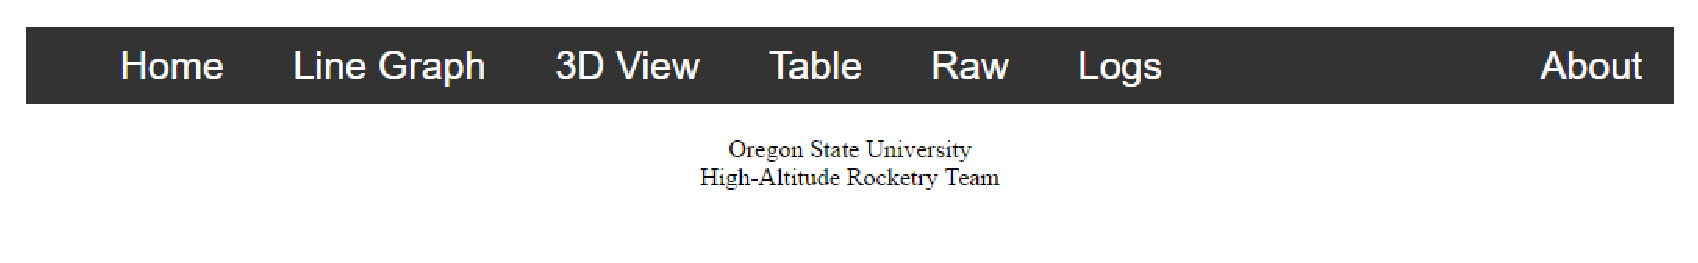
\includegraphics[width=170mm]{gs-header}
		\caption{The home screen}
		\label{gs-home}
	\end{figure}
	
Figure~\ref{gs-home} shows the home screen.
This screen is the page that is loaded when the user navigates to the web page.
THe home screen is intentionally lightweight to allow the user to get to
the page they want faster.
Clicking the various links on the top of the page will navigate to the various views.

\subsubsection{Line Graph}
	\begin{figure}[thbp!]
		\centering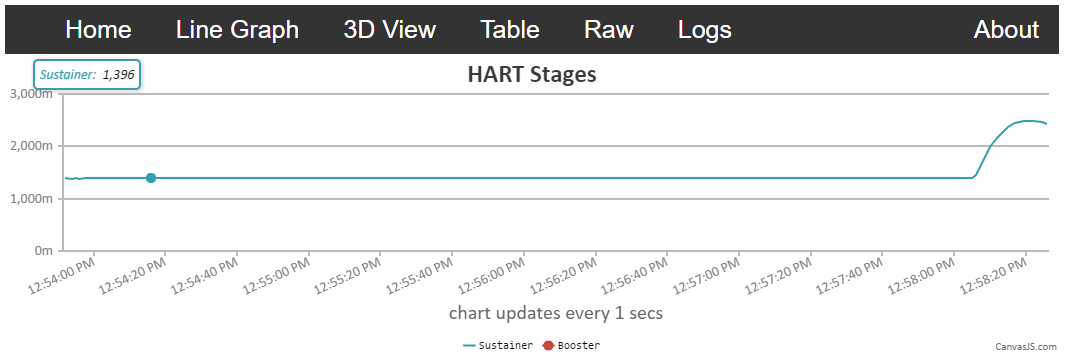
\includegraphics[width=170mm]{gs-line}
		\caption{The line graph}
		\label{gs-line}
	\end{figure}
	
Figure~\ref{gs-line} shows the line graph.
This is a graph of the current altitude for both the booster and the sustainer.

\subsubsection{3D View}
	\begin{figure}[thbp!]
		\centering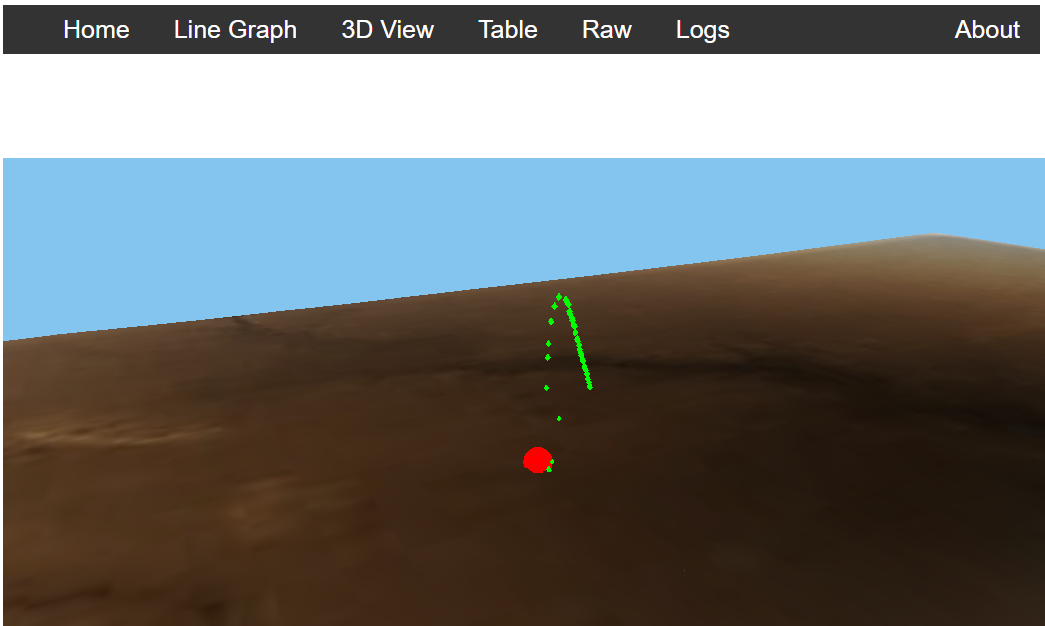
\includegraphics[width=170mm]{gs-3d}
		\caption{The 3D view}
		\label{gs-3d}
	\end{figure}
The 3D view, shown in figure~\ref{gs-3d}, plots the rocket's position in three dimensions in real-time.
The trail of green dots show where the rocket has been, and the red dot shows the position of the launch pad.
Hold down the right mouse button to rotate the camera, and use the mouse wheel to zoom in and out.

\subsubsection{Table View}
	\begin{figure}[thbp!]
		\centering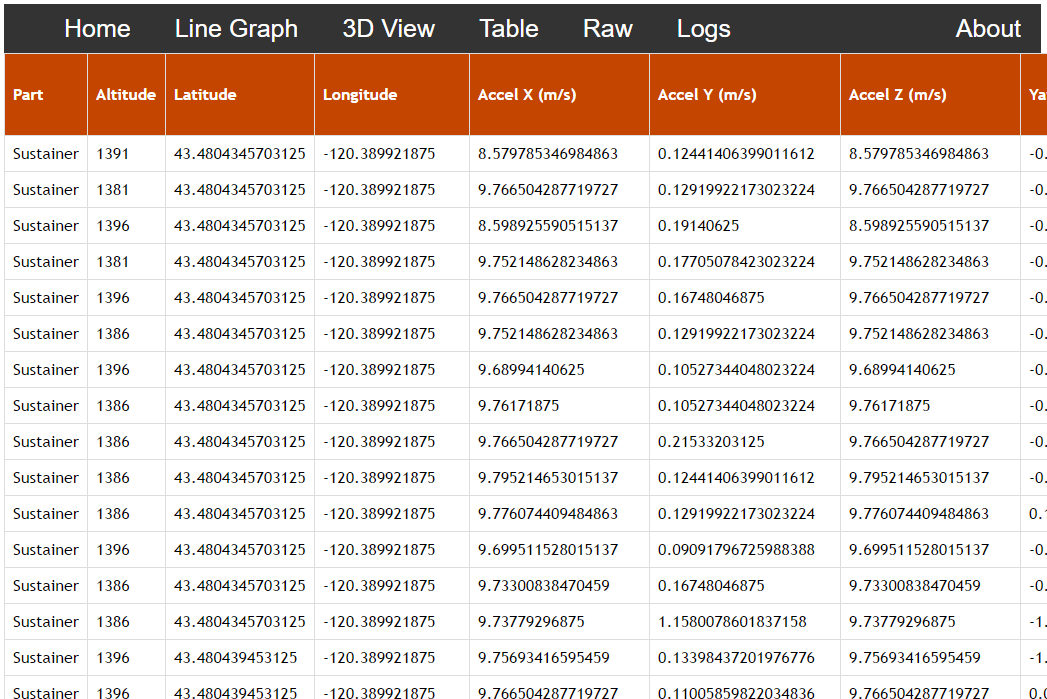
\includegraphics[width=170mm]{gs-table}
		\caption{The table view}
		\label{gs-table}
	\end{figure}
The table view (figure~\ref{gs-table}) allows the user to view all data that was collected since
the groundstation was turned on.
New rows are added to the bottom of the table as packets are recieved.
In order to prevent browser slow-down, table updating is limited to once per second,
even if telemetry is being received at a higher rate.

\subsubsection{Raw View}
	\begin{figure}[thbp!]
		\centering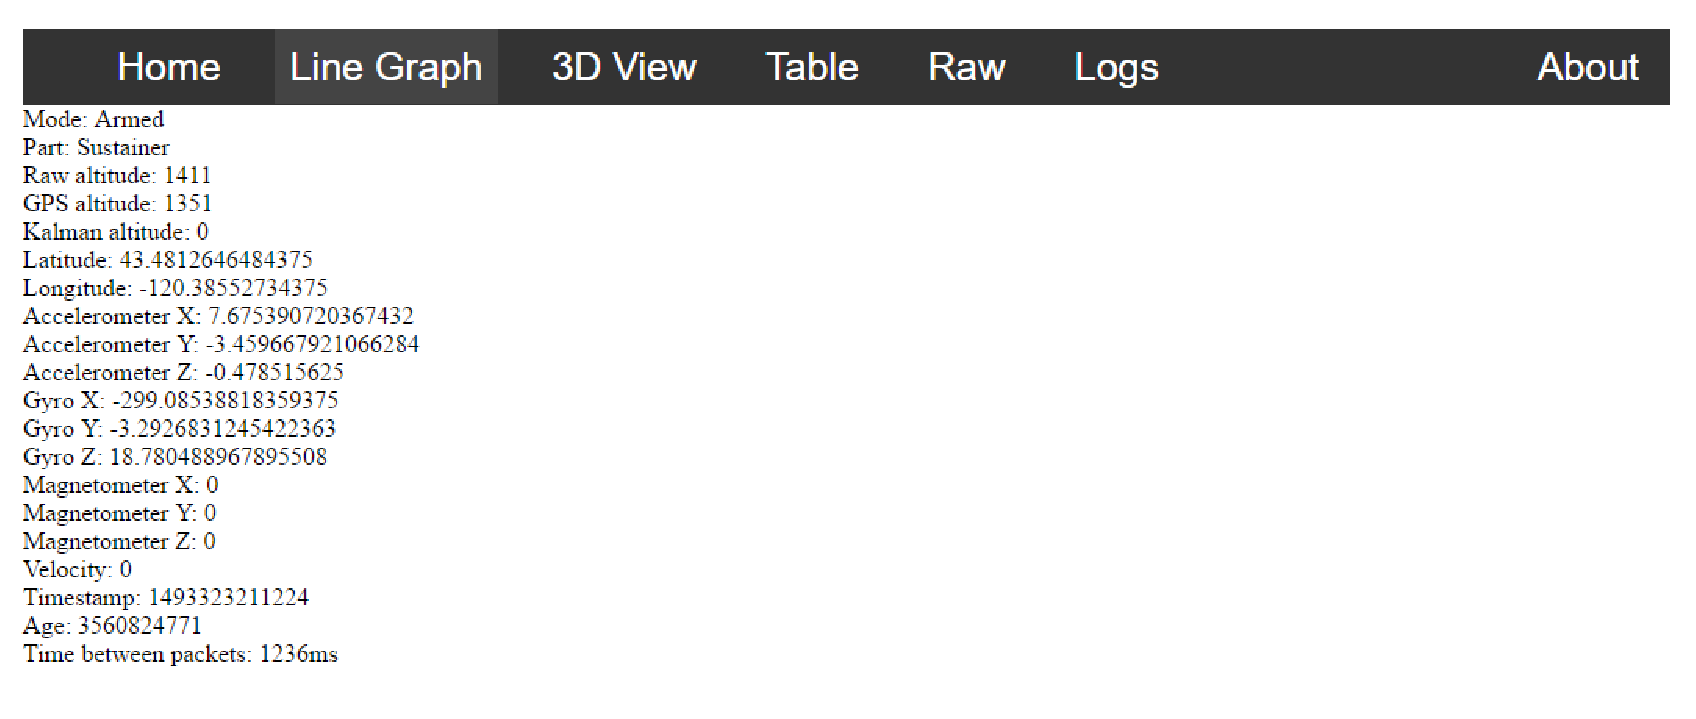
\includegraphics[width=170mm]{gs-raw}
		\caption{The raw view}
		\label{gs-raw}
	\end{figure}
The raw view, shown in figure~\ref{gs-raw}, shows all of the most recent telemetry from both the
booster and the sustainer. All units are in degrees or meters, as appropriate.
Altitude is listed in meters above sealevel (not groundlevel).
``Raw altitude'' shows the altitude from the barometric sensors onboard the rocket,
and ``GPS altitude'' reports the altitude from the global positioning system.
``Timestamp'' shows the current time in milliseconds since January 1, 1970.
Note ``Age'' property shows the age of packets, but it calculated by comparing the
web browser's time to the server's time.
If the web browser's and server's time are not synchronized, then the ``Age'' field will
never reach zero.
However, this field is useful for telling when the data is ``caught up'' to the present,
and all historical telemetry has been sent.
If the age is rapidly decreasing, then historical telemetry is still being sent.


\subsubsection{Download Logs}
	\begin{figure}[thbp!]
		\centering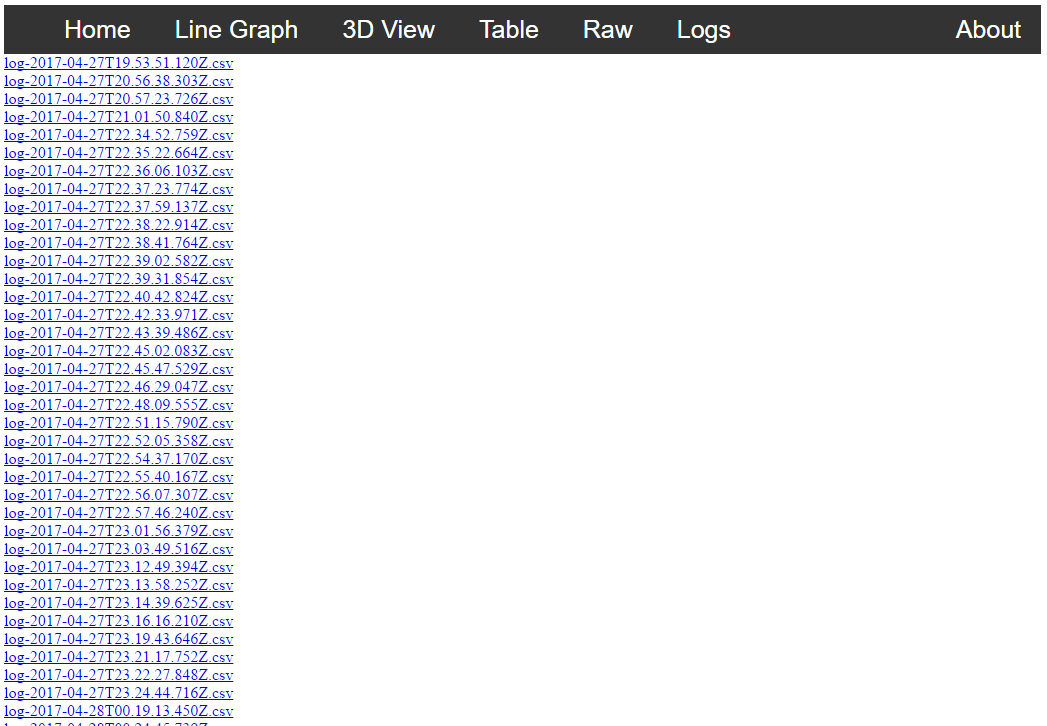
\includegraphics[width=170mm]{gs-logs}
		\caption{The logs download page}
		\label{gs-logs}
	\end{figure}
Figure~\ref{gs-logs} shows logs page.
Every time the groundstation is powered on, a new log file is created.
The filename of each log is the current time in UTC.
Users may simply click on the log that corresponds to the time of the launch to download data for that time.
All log files are in CSV files and may be loaded natively in applications such as Microsoft Excel.
	






















% CHAPTER
% LEARNING TECHNOLOGY

\newpage
\section{How We Learned New Technology}

\subsection{Anisimova, Natasha}

% Natasha's learning stuff here

\subsection{Lee, Terrance}

% An old dog can be taught new tricks

\subsection{Morgan, Albert}

% What I learned in kindergarten today.








































% CHAPTER
% LEARNING TECHNOLOGY

\newpage
\section{What We Learned}

\subsection{Anisimova, Natasha}

% Natasha's learning stuff here

\subsection{Lee, Terrance}

% An old dog can be taught new tricks

\subsection{Morgan, Albert}

% What I learned in kindergarten today.





















% APPENDIX 1
\newpage
\appendix[Code Listings]



	
\printindex
\bibliography{final}
\bibliographystyle{IEEEtran}
\end{document}
